\documentclass[12pt,oneside,a4paper]{article}
\title{Shark biomimetics: Drag reduction beyond parallel riblets.
\\
 Transfer report
}
\author{Charlie Lloyd : sccjl@leeds.ac.uk
\\\\
\textit{Supervised by}
\\
Professor Jeff Peakall, Dr Alan Burns,
\\
Dr Gareth Keevil, and Dr Robert Dorrell.
\\\\}

\usepackage[margin=1in]{geometry}
\usepackage{graphicx}
\usepackage{xcolor}
\usepackage{enumitem}
\usepackage{setspace}
\usepackage[british]{babel}
\usepackage{natbib}
\usepackage{multirow}
\usepackage{caption}
\usepackage[mathscr]{euscript}

\DeclareCaptionFormat{cont}{#1 (cont.)#2#3\par}
\newcommand*{\vcenteredhbox}[1]{\begingroup
\setbox0=\hbox{#1}\parbox{\wd0}{\box0}\endgroup}

\bibliographystyle{apalike}

\usepackage{siunitx}


\onehalfspacing

%%%%%%%%%%%%%%%%%%%%%%%%%%%%%%%%%%%%%%%%%%%%%%%%%%%%%%%%%%%%%%%%%%%%%%%
%%%%%%%%%%%				MATHS COMMANDS			%%%%%%%%%%%%%%%%%%%%%%%
\usepackage{amssymb,amsmath, amsbsy, mathalfa}


\newcommand{\av}[1]{\overline{#1}}
\newcommand{\pdev}[2]{\frac{\partial {#1}}{\partial {#2}}}
\newcommand{\Ddev}[2]{\frac{D {#1}}{D {#2}}}
\newcommand{\ldev}[2]{\frac{D {#1}}{D {#2}}}
\newcommand{\vect}[1]{\boldsymbol{#1}}
\newcommand{\vecti}[1]{{#1}_{i}}
\newcommand{\vectj}[1]{{#1}_{j}}
\newcommand{\vectk}[1]{{#1}_{k}}
\newcommand{\mat}[1]{\boldsymbol{#1}}
\newcommand{\matij}[1]{{#1}_{ij}}
\newcommand{\matji}[1]{{#1}_{ji}}
\newcommand{\divv}{\nabla}
\newcommand{\vectfi}[1]{{#1}_{f,i}}
\newcommand{\vectfj}[1]{{#1}_{f,j}}
\newcommand{\vectfk}[1]{{#1}_{f,k}}
\newcommand{\vectpi}[1]{{#1}_{p,i}}
\newcommand{\vectpj}[1]{{#1}_{p,j}}
\newcommand{\vectpk}[1]{{#1}_{p,k}}
%%%%%%%%%%%%%%%%%%%%%%%%%%%%%%%%%%%%%%%%%%%%%%%%%%%%%%%%%%%%%%%%%%%%%%%

\begin{document}
\pagenumbering{gobble}
\maketitle



\newpage

\tableofcontents

\newpage
\pagenumbering{arabic}
\section{Introduction}
\cite{dean2010} define biomimcry as the study of naturally occurring properties of plants and animals for the purpose of inspired design. This particular project investigates how we can reduce the fluid dynamic drag that acts on surfaces, such as ship hulls and aircraft wings, by investigating animals that swim long distances in the ocean. There are several natural mechanisms that have evolved to reduce drag, such as the excretion of mucus, but sharks posses a unique method that can be theoretically replicated and applied to smooth surfaces \citep{dean2010}. Sharks have evolved dermal denticles (skin teeth) which help the fish defend against parasites, abrasion, and reduce hydrodynamic drag \citep{fletcher2014}. While the hydrodynamic benefit of shark scales has been known for decades, most work has been focussed on the riblet features that exist on the crest of fast-swimming shark scales, examples of which can be observed in Figure \ref{figure:scalesExample}. These riblets have been simplified and applied to open and closed channel flows and aerofoils, typically achieving a maximum drag reduction of $\sim 10\%$ \citep{dean2010}.
\begin{figure}[!b]
\centering
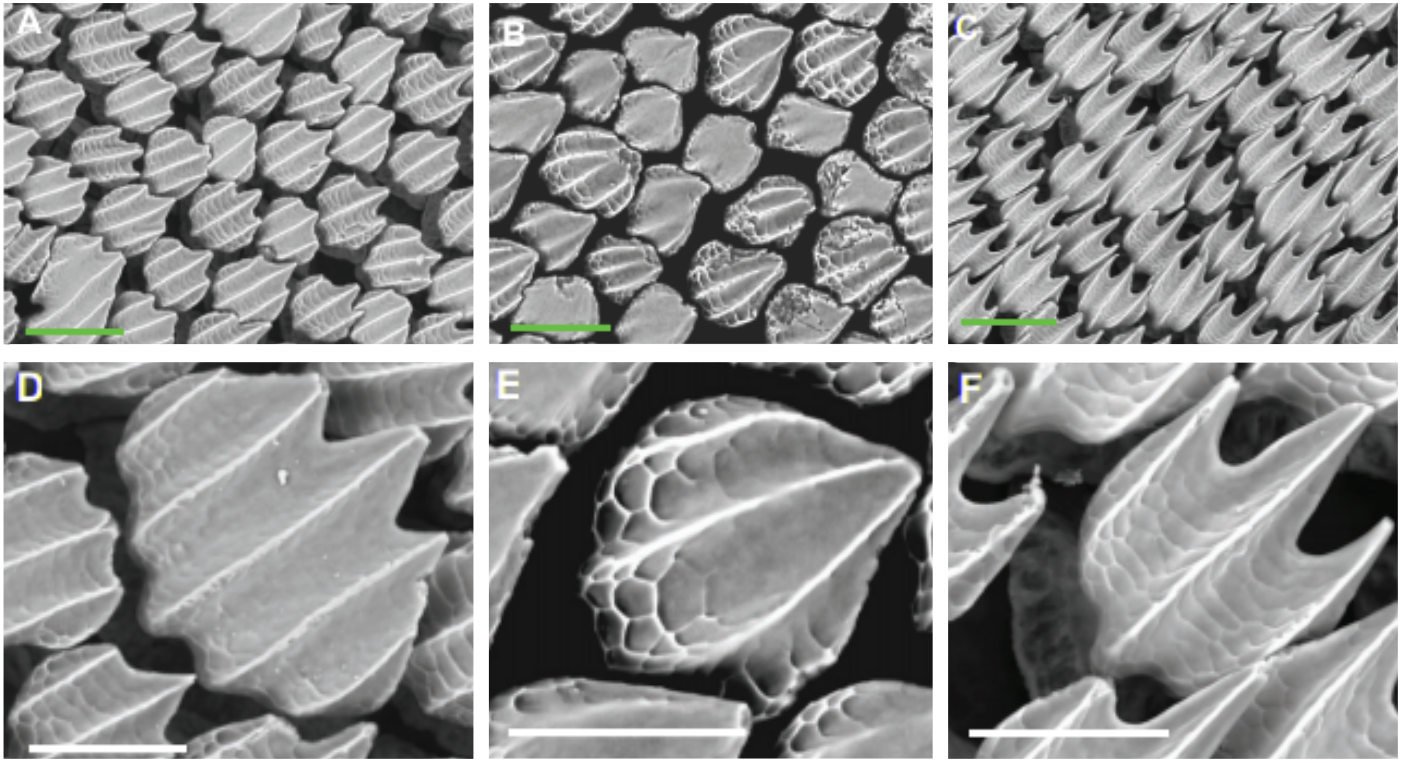
\includegraphics[width=12cm]{images/Scales2.png}
\caption{Shark scale samples taken from the head (A, D), the dorsal fin (B, E), and the anal fin (C, F) of a Mako shark. Green scale bars are \SI{200}{\mu m}; white scale bars are \SI{100}{\mu m}. Image adapted from \cite{wen2014}.}
\label{figure:scalesExample}
\end{figure}

However, riblets are one of many features that are present on shark scales (see Figure \ref{figure:scalesExample}). Through observation of the surface it is clear that the scales are very three-dimensional and variable in geometry between different shark species and location on the shark \citep{fletcher2014phd}. Some shark species have scales with no riblets, loosely interlocking scales, and variable angles of attack \citep{fletcher2014phd}. The dermis, of which scales are embedded, is known to be flexible, but the effect of this on the flow is not yet well understood \citep{wen2014}. The limited amount of work that has been carried out on shark scale surfaces is much more contradictory than similar experiments on riblets. This is due to variations in the scale geometry, replication errors, and experimental conditions. In addition to this, the most common experimental techniques are limited by the use of force balances, reducing the complexity of the flow to a single drag coefficient (further discussed in Section \ref{section:literatureReview}).


%Detailed flow structures have been investigated by either increasing the  size of the scales by several orders of magnitude \citep{lang2008} or carrying out expensive direct numerical simulation \citep{boomsma2015}.





\subsection{Research questions}

This project aims to determine the effect of scale geometry on the flow in order to identify why certain features have evolved and whether they can be optimised for drag reduction. In particular, the project aims to identify the effects of scale height and width, spacings between scales, the addition of riblets to smooth scales, and the effect of altering the angle of attack. This will be achieved by applying numerical parametric methods to a periodic array of scales. This will be validated against both a Large-Eddy Simulation (LES) and laboratory experiment utilising Laser Doppler Anemometry (LDA).
 
In addition to this the project will investigate the effect of applying scales to surfaces subject to separating flows. It has long been theorised that scales may prevent flow separation \citep{bechert1985} but current research is limited to analysis of large scale flow structures, rather than the flow features around individual scales. LES will be applied to a separating flow in order to quantify the differences between smooth and shark-skin surfaces. The results will be validated against a laboratory experiment using Particle Image Velocimetry (PIV). 

Despite the potential resolution of numerical methods, they have so far seen little use for resolving the flow around shark scales. This project will primarily use these techniques, validated against experimental data.

\subsection{Aim and Objectives}
\label{section:AandO}

There are two aims of this project; to investigate the influence of shark scale geometry on a fully developed flow, and to investigate the impact of scales on separating flows. Both of these aims will primarily concern the flow fields close to/around the scales. These will be achieved through completion of the following objectives:
\begin{itemize}
\itemsep0em

\item Identify experimental and numerical methods currently used in the literature and investigate their applicability to the current project.

\item Investigate potential software packages in terms of Computer-Aided Design (CAD) and Computational Fluid Dynamics (CFD). Carry out preliminary tests on potential software and identify which are most suitable. 

\item Carry out 3D LDA experiments for an array of scales in a channel.

\item Carry out a high resolution LES for the same array of scales and validate against LDA data. 

\item Validate a parametric RANS code against the LES/LDA data and carry out a parametric analysis on the effect of scale geometry on the fluid flow. 

\item Design and carry out laboratory (PIV) and numerical experiments (TBC) that can be used to investigate the influence of shark scales on separating flows.  

\end{itemize}

\newpage
\section{Literature Review}
\label{section:literatureReview}

%\subsection{Shark scales}
%\label{section:literatureReview:sharkScales}
Sharks are the only surviving fishes that possess dermal denticles \citep{fletcher2014phd}. These small tooth-like structures erupt through soft skin tissue and are optimised for the prevention of abrasion, defence against parasites, and the reduction of hydrodynamic drag \citep{fletcher2014phd}. An extensive range of dermal denticles are documented by \cite{reif1985}, highlighting the differences between shark species and the location of scales on the fishes. The study also indicates the complex features of real shark scales such as three dimensionality beneath the exposed scale, overlapping, diverging and converging riblets, variable angles of incidence, and the aerofoil-like shape of each scale with a smooth leading edge and a sharp trailing edge. These features can be observed in Figure \ref{figure:literatureReview:scaleVariabilityFletcher};
\begin{figure}[!b]
\centering
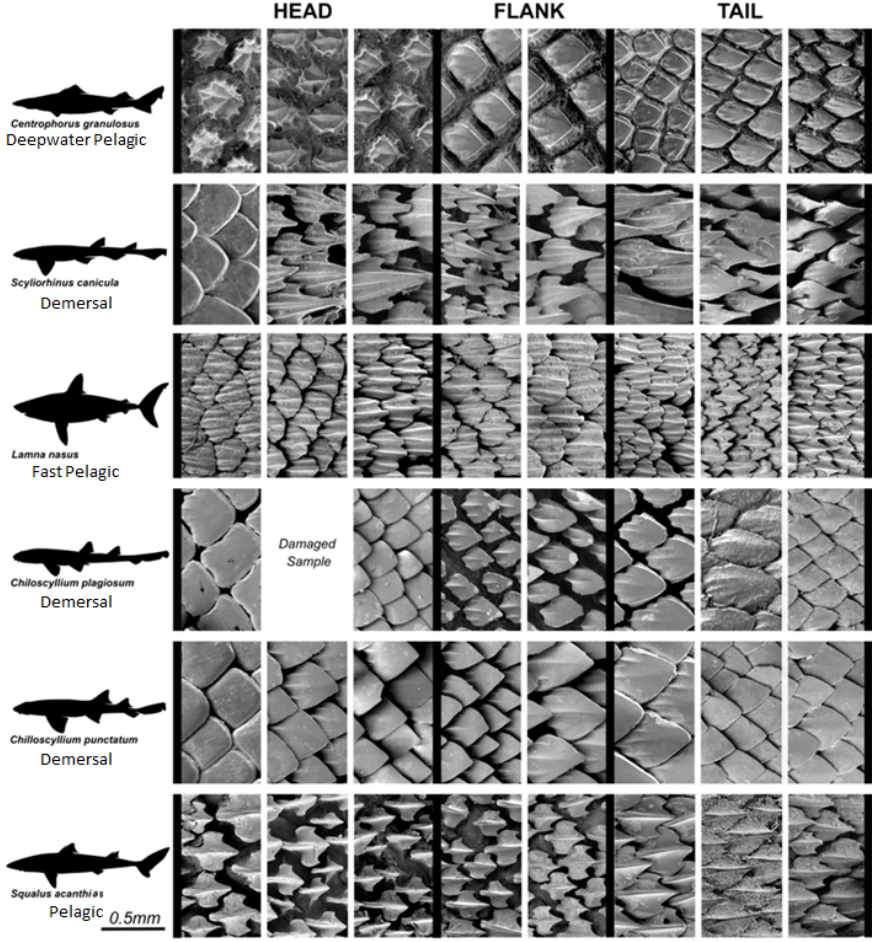
\includegraphics[width=14cm]{images/litReview/scaleVariabilityFletcher.png}
\caption{The variation of denticles between six fish species. Image taken from \citep{fletcher2014phd}.}
\label{figure:literatureReview:scaleVariabilityFletcher}
\end{figure}
even when considering just one species the scales can vary significantly when moving from the head to the tail. Take, for example, the \textit{Scyliorhinus canicula} (demersal ecology) samples in Figure \ref{figure:literatureReview:scaleVariabilityFletcher}; the scales on the head of the shark are tightly interlocking and rounded scales which quickly change to sharp, loosely interlocked, and ribletted scales on the sharks flank. The vast range of these features, and the variability between species, results in little understanding as to why many of these features exist. Hydrodynamical aspects have only been studied over the last few decades \citep{dean2010} and have mainly focussed on riblets, examples of which are most prominent on the fast pelagic samples of Figure \ref{figure:literatureReview:scaleVariabilityFletcher}. There has been research into the fluid dynamics of shark scales but there are many gaps and inconsistencies in the literature. These will be discussed in Section \ref{section:literatureReview:sharkScaleFluids}.
%Before reviewing the experiments carried out on shark scales and riblets we must first understand the underlying principles behind boundary layers and skin friction. 
%
\subsection{Boundary layers and skin friction}
Most engineering and atmospheric flows are bounded by one or many surfaces. These take the form of external flows, such as the flow around cars and aircraft, and internal flows, such as through pipes and channels. Boundary layers are formed as a fluid passes over a surface, whereby the fluid velocity converges to zero as the distance to the wall decreases. Skin friction, arising from the no-slip condition, can be a large contribution to the total drag force that impedes the motion of an object: \SI{50}{\%} of the drag that acts on a ship hull is due to skin-friction \citep{perlin2016}. A typical boundary layer is presented in Figure \ref{figure:literatureReview:boundaryLayerRegions}, which splits the temporally averaged streamwise velocity into several different regions.
%
\begin{figure}[!b]
\centering
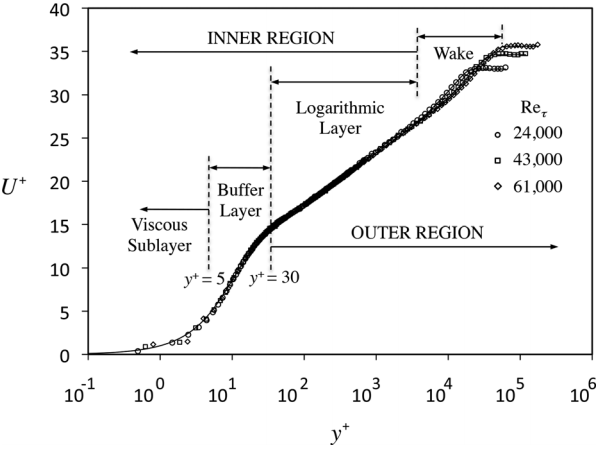
\includegraphics[width=10cm]{images/litReview/boundaryLayerRegions.png}
\caption{Typical boundary layer profile for three Reynolds numbers. Image taken from \cite{perlin2016}. }
\label{figure:literatureReview:boundaryLayerRegions}
\end{figure}
%
The velocity and spatial variables are scaled using the fluid kinematic viscosity, $\nu$, and friction velocity, $u_\tau = \sqrt{\tau_w / \rho}$, where $\tau_w$ is the wall shear stress and $\rho$ is the fluid density:
\begin{equation}
U^+ = \frac{U}{u_\tau}, \hspace{1cm} y^+ = \frac{u_\tau y }{\nu}.
\end{equation}
By using this scaling the velocity profiles of many external and internal flows behave in the way indicated by Figure \ref{figure:literatureReview:boundaryLayerRegions}, whereby the boundary layer is split into external and internal regions. The inner region consists of a viscous sub-layer, a buffer layer, and a logarithmic layer. When in the viscous sub-layer the streamwise (wall-parallel) velocity of a fluid is proportional to the distance away from it, such that $U^+ = y^+$. This extends until $y^+ \approx 5$, at which point the production of turbulent kinetic energy rapidly increases until reaching its maximum in the buffer layer \citep{perlin2016}. The logarithmic region begins at $y^+ \approx 30$, at which point the streamwise velocity behaves like $U^+ = \kappa^{-1} \ln{y^+} + B$ where $\kappa \approx 0.4$ is the von Karmon constant and $B\approx 5$ is the intercept parameter \citep{pope2001}.

The outer layer blends the logarithmic region into the freestream velocity. The wake region, identified by Figure \ref{figure:literatureReview:boundaryLayerRegions}, deviates from the log-law and can cover a large amount of the boundary layer. For an external flow the wake region typically exists for $y/\delta^* > 0.2$ where $\delta^*$ is the boundary layer thickness, defined as the point at which the mean streamwise velocity is equal to \SI{99}{\%} of the freestream velocity, $U_\infty$ \citep{pope2001}. Surface roughness, including shark scales, have no effect on the wake portion of the outer boundary layer \citep{flack2010}.

Relationships between the skin friction drag and the flow field can be derived from the Reynolds equations \eqref{equation:literatureReview:ReynoldsEquations} and the continuity equation \eqref{equation:literatureReview:Continuity} \citep{pope2001}:
\begin{equation}
\pdev{\langle U_i \rangle}{t} + \langle U_j \rangle \pdev{\langle U_i \rangle}{x_j}
=
-\pdev{\langle P \rangle}{x_i}
+
\nu
	\left(
	\pdev{\langle U_j \rangle}{x_i}
	+
	\pdev{\langle U_i \rangle}{x_j} 
	\right)
-
\pdev{\langle u_i u_j\rangle}{x_i},
\label{equation:literatureReview:ReynoldsEquations}
\end{equation}
and 
\begin{equation}
\pdev{\langle U_i \rangle}{x_i}
=
0,
\label{equation:literatureReview:Continuity}
\end{equation}
where the three component velocity vector, $U_i$, and the kinematic pressure, $P$, are decomposed into an ensemble mean and fluctuating component: $U_i = \langle U_i \rangle + u_i$, and $P = \langle P \rangle + p$. $\langle u_i u_j \rangle$, is termed the Reynolds stresses which account for the effect of velocity fluctuations on the mean flow \citep{pope2001}. The FIK identity \citep{fukagata2002} manipulates \eqref{equation:literatureReview:FIK} to determine a relationship for the coefficient of skin friction. For a statistically steady and fully developed channel flow the FIK identity reduces to
\begin{equation}
\label{equation:literatureReview:FIK}
C_f = \frac{\tau_w}{\frac{1}{2} \rho U_b^2} = \frac{12}{Re_b} + 12 \int_0^\delta 2 \left(1 - \frac{y}{\delta} \right)\left( - \frac{\left< u_x u_y \right> }{4 U_b^2} \right) dy,
\end{equation}
where $C_f$ represents the coefficient of friction and $Re_b$ is the bulk Reynolds number based on the bulk velocity, $U_b$, and the channel half height, $\delta$. Similar equations can also be derived for pipe flows and flat plates. \cite{newhall2006} derives an integrated boundary layer equation, similar to \eqref{equation:literatureReview:FIK}, to compare the skin friction coefficients for smooth and rough flat plate flows. 

By setting the Reynolds stresses to zero it is clear that \eqref{equation:literatureReview:FIK} is decomposed into a laminar and turbulent component \citep{kasagi2006}. It is the reduction of this turbulent component that is key to how riblets reduce drag, as will be discussed in Section \ref{section:literatureReview:Riblets}.

\subsection{Surface roughness}
\label{section:literatureReview:roughness}
The majority of real engineering problems are subject to surface roughness which generally increases skin friction. The first quantitative study on the effect of surface roughness was carried out by \cite{nikuradse1933} who applied different grain sizes of sand to a pipe flow and measured the resulting friction factor (equivalent to the coefficient of friction, $C_f$). \cite{nikuradse1933} observed that for laminar, and transitional flows, surface roughness had little effect, and its effect on fully turbulent flows was dependent on the relative size of the roughness. To describe the effect of roughness on turbulent flows three regimes were defined, based on the average roughness height, $k_s$:
%
$$\frac{k_s u_\tau}{\nu} < 5: \text{Hydraulically smooth,} $$
$$5 \leq \frac{k_s u_\tau}{\nu} \leq 70:	\text{transitionally rough,} $$
$$70 < \frac{k_s u_\tau}{\nu}:	\text{fully rough.}		$$
%
The hydraulically smooth regime occurs when the roughness elements do not protrude above the viscous sub-layer; in this case roughness has no effect. During the transitional stages roughness elements begin to protrude beyond the viscous sub layer, creating additional turbulent mixing and form drag on individual elements; both of these effects increase the friction factor relative to a smooth surface. The effect of roughness continues to grow until entering the fully-rough regime, at which point the friction factor is no longer a function of the Reynolds number.

In terms of the mean velocity profile, roughness has the effect of shifting the logarithmic layer towards the wall such that the velocity behaves like
\begin{equation}
\label{equation:litReview:roughLawOfWall}
U^+ = \frac{1}{\kappa} \ln{y^+} + B - \Delta U^+,
\end{equation}
where $\Delta U^+$ represents the shift \citep{newhall2006}. The gradient of the logarithmic region remains the same for both smooth and rough surfaces. In addition to this the outer layers of the boundary experience no change when subject to surface roughness, despite there being an increase to the boundary layer thickness, $\delta^*$ \citep{perlin2016}.
%However, the above description does not hold true for all types of roughness. In particular, the effect of shark-skin, and shark-skin inspired riblets, have a very different effect on the flow. These will be discussed in sections \ref{section:literatureReview:Riblets} and \ref{section:literatureReview:sharkScaleFluids}.

\subsection{Riblets}
\label{section:literatureReview:Riblets}
An extensive amount of work has been carried out on simplified, sharkskin-inspired, riblets which have been successful in reducing drag for open channel flows, closed channel flows, and when applied to aerofoils \citep{bixler2013review}. These riblets are generally two-dimensional, whereby there is no variation in cross section in the streamwise direction. The most popular cross sectional shapes are blade-like, sawtooth, and scalloped, although they are theorised to reduce drag in the same way. An example of blade-like riblets is presented in Figure \ref{figure:literatureReview:bladeRiblets}, and when compared to the denticle samples of Figure \ref{figure:literatureReview:scaleVariabilityFletcher} it is clear that the intricate details present on real shark scales are lost.
%
\begin{figure}[!b]
\centering
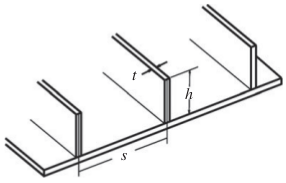
\includegraphics[width=8cm]{images/bladeRiblets.png}
\caption{An example of blade-like riblets. Image taken from \cite{dean2010}.}
\label{figure:literatureReview:bladeRiblets}
\end{figure} 
%
Riblets are typically characterised by their spacing in wall units, $s^+ = u_\tau s / \nu$, although other length scales have been suggested. For example, \cite{garcia2011a} proposes a scaling based on the cross-sectional groove area, $(A_g^+)^{1/2}$. The performance of a typical ribletted surface is presented in Figure \ref{figure:literatureReview:ribletPerformanceRegions}, whereby the difference in wall shear stress, $\Delta \tau / \tau_0$, is plotted against the dimensionless riblet spacing, $s^+$.
%
\begin{figure}[!t]
\centering
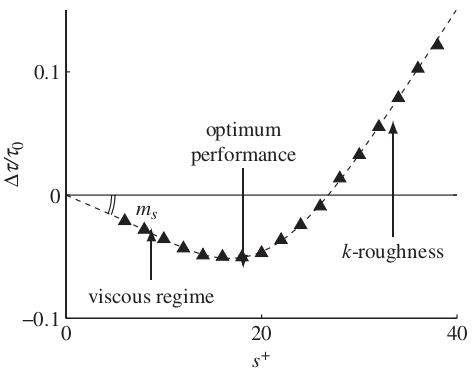
\includegraphics[width=8cm]{images/litReview/ribletPerformanceRegions.png}
\caption{A typical drag reduction profile for a ribletted surface. Image taken from \cite{garcia2011}.}
\label{figure:literatureReview:ribletPerformanceRegions}
\end{figure}
%
The viscous regime exists for riblets with a spacing of $s^+  \lesssim 15$ whereby the drag reduction scales linearly with spacing. For a small riblet spacing the riblets are submerged in the viscous sub-layer. Realising this, \cite{luchini1991} used the two-dimensional linear Stokes equations to investigate the flow field. The performance of a particular riblet geometry was found to be related to its virtual origin, whereby the riblet surface can be represented by a flat plate whose origin lies somewhere below the riblet tips. \cite{luchini1991} determined that the virtual origin of spanwise flow lies deeper in the riblet than for streamwise flow. The difference between these two origins  is termed the protrusion height, $\Delta h$. \cite{luchini1991} argued that the larger the protrusion height, the larger the restriction on spanwise flow that could otherwise lead to turbulent mixing above the riblets. This theory is supported by the inhibition of near-wall low speed streaks observed by \cite{chu1993}, and the study of \cite{yang2016} who observed a reduced number of sweep and ejection events over a ribletted surface which are known to be large contributors to turbulent mixing \citep{pope2001}.

A commonly cited empirical relationship predicting the drag reduction of a ribletted surface was derived by \cite{bechert1997}:
\begin{equation}
\label{equation:literatureReview:ribletGradient}
\frac{\Delta \tau}{\tau_0} = m_s s^+ = - \frac{\mu_0 (\Delta h / s)}{(2 C_f)^{-1/2} + (2 \kappa)^{-1}}s^+,
\end{equation}
where $m_s$ is the gradient indicated by Figure \ref{figure:literatureReview:ribletPerformanceRegions} and $\mu_0 = 0.785$ is an empirical constant. The roughness parameter of 
\eqref{equation:litReview:roughLawOfWall} is related to the protrusion height by $\Delta U^+ = - \mu_0 \Delta h^+$, such that the mean velocity profile is shifted away from the wall, contrary to typical rough surfaces. This theory provides a reasonable estimation for the performance of small riblet spacings; through Direct Numerical Simulation (DNS) \cite{garcia2011a} identified a stable spanwise recirculation pattern inside the riblet spacing that mimicked those of a two-dimensional linear stokes solution. This recirculation pattern became increasingly unstable and asymmetric as the spacing increased. At the optimal region, \cite{garcia2011a} identified the formation of large spanwise vortices, above the riblet tips, due to a Kelvin-Helmholtz type instability. The same vortices were identified in further simulations at a Reynolds number of $Re_\tau = u_\tau \delta / \nu = 550$ \citep{garcia2012}. \cite{garcia2012} also suggest that simulations at low Reynolds numbers of $Re_\tau = 180$, commonly observed in the literature, are equally valid for the study of surface roughness as higher Reynolds numbers, despite perhaps not being as representative of the flow conditions for practical applications. 

As the dimensionless riblet spacing increases the riblets begin to interact with layers above the viscous sub-layer and the predictions of \eqref{equation:literatureReview:ribletGradient} deviate from experiments. The region after the optimum performance behaves like k-roughness, whereby the roughness parameter can be represented by $\Delta U^+ = \kappa^{-1} \ln k_s + A$, where the roughness height, $k_s$, is related to the dimensions of the riblet \citep{jimenez2004}. As the riblet spacing increases, they lose their ability to constrict spanwise flow and fast moving fluid can penetrate to the base of the grooves, as observed by \cite{lee2001}. 

The application of riblets to adverse pressure gradients (APG) is still an area of much uncertainty \citep{boomsma2015}. Tables \ref{table:litReview:openChannelRiblets} and \ref{table:litReview:ribletsAerofoil} indicate the discrepancies between the application of riblets to channel flows and aerofoils.
%
\begin{table}[!t]
\scriptsize
\centering
\caption{Summary of experimental literature concerning the application of riblets to open channel flows. Adapted from \cite{bixler2013review}.}
\label{table:litReview:openChannelRiblets}
\begin{tabular}{|l|l|l|c|l|}
\hline
& & & & \\
\small Design                                                          & \small Confirguration                                            & \small Material                                              &  \multicolumn{1}{|l|}{\small Maximum Drag} &\small  Reference \\
& & & \multicolumn{1}{|l|}{\small Reduction} & \\
\hline
%
Sawtooth	& Continuous	& Polymer	& 8\%	& \citep{reidy1988}		\\
Sawtooth	& Continuous	& Vinyl		& 9\%	& \citep{rohr1992}		\\
Sawtooth	& Continuous	& Vinyl		& 6\%	& \citep{walsh1990}		\\
Sawtooth	& Continuous	& Vinyl		& 9\%	& \citep{neumann1991}	\\
%
%
\begin{tabular}[c]{@{}l@{}}Blade, Sawtooth\\ \& Scalloped\end{tabular} & Continuous	& Brass		& 9.9\%	& \citep{bechert1997}	\\
%
%
Blade		&	\begin{tabular}[c]{@{}l@{}}Staggered\\ \& Segmented\end{tabular}	& Brass		& 7\%	& \citep{bechert2000}	\\
Blade		&	\begin{tabular}[c]{@{}l@{}}Staggered\\ \& Segmented\end{tabular} 	& Epoxy		& 7\%	&	\citep{bechert2000}	\\
%
%
Blade		& Continuous	&	\begin{tabular}[c]{@{}l@{}}Titanium \&\\ Nickel\end{tabular}		& 4.9\%		&	\citep{buttner2011}	\\
%
%
Sawtooth	& Continuous	& Polyurethane		& 7.6\%		&	\citep{gruneberger2011}	\\
%
%
Blade		& Continuous	& \begin{tabular}[c]{@{}l@{}}Metal \&\\ Polymer\end{tabular}	& 8.5\%		&   \citep{wilkinson1988}	\\
%
%
Sawtooth, Scalloped		& Continuous	& \begin{tabular}[c]{@{}l@{}}Aluminium \&\\ Vinyl\end{tabular}	& 8\%	&  \citep{walsh1982}  \\ \hline 
\end{tabular}
\end{table}
%
%
\begin{table}[!b]
\centering
\scriptsize
\caption{Summary of experimental literature concerning the application of riblets on aerofoils. Adapted from \cite{bixler2013review}.}
\label{table:litReview:ribletsAerofoil}
\begin{tabular}{|l|l|l|l|c|l|}
\hline
\begin{tabular}[c]{@{}l@{}}\small Reynolds\\\small Number\end{tabular}  &\small Foil Type                                                 & \begin{tabular}[c]{@{}l@{}}\small Location of\\\small  Trip (\% Chord\\ \small  Length)\end{tabular} & \begin{tabular}[c]{@{}l@{}} \small Angle of\\ \small  Attack\\ \small (degrees)\end{tabular} & \multicolumn{1}{|l|}{\begin{tabular}[c]{@{}l@{}} \small Maximum Drag\\ \small Reduction\end{tabular}} & \small Reference \\
\hline
17000	& \begin{tabular}[c]{@{}l@{}}Symmetric,\\ Thin\end{tabular}	& No Trip	& 0			& 4.3\%		& \cite{han2003}			\\
250000	& \begin{tabular}[c]{@{}l@{}}Symmetric,\\ Thin\end{tabular} & No Trip	& 0			& 13.3\%	& \cite{caram1991}			\\
750000	& Thin                                                      & 10\%		& 0-6		& 6\%		& \cite{sundaram1999}		\\
1000000	& Symmetric                                                 & 10\%		& 0-6		& 13\%		& \cite{sundaram1996}		\\
1000000	& Thin                                                      & 5\%		& 0			& 14\%		& \cite{subaschandar1999}	\\
1000000	& Thick                                                     & No Trip	& 0			& 5\%		& \cite{wetzel1996}     	\\
\begin{tabular}[c]{@{}l@{}}1000000\\ -1850000\end{tabular} & Thick	& No Trip	& 0			& 5\%		& \cite{sareen2011}    		\\
3000000	& Thick                                                     & 6\%		& -0.5-1	& 10\%		& \cite{viswanath1995}		\\
3300000	& Thin                                                      & No Trip	& 0			& 3.3\%		& \cite{coustols1990}      	\\
\begin{tabular}[c]{@{}l@{}}2000000\\ -6000000\end{tabular} & \begin{tabular}[c]{@{}l@{}}Symmetric,\\ Thin\end{tabular}
																	& 5\%		& 0			& 7\%		& \cite{bixler2013review}	\\
\hline   
\end{tabular}
\end{table}
%
%
 Even when taking into account the different configurations and riblet types, open channel flow experiments indicate a range of only \SI{5}{\%} for the maximum drag reduction. When riblets are applied to aerofoils the range increases to \SI{10}{\%}. This is largely due to the additional dependencies on riblet configuration and the shape of the foil; the experiments of \cite{chamorro2013}, carried out on a wind turbine blade, indicate that for some cases a partially ribletted foil reduces drag more than a fully covered foil. This is due to development of the boundary layer over the foil; unlike the fully turbulent channel flow experiments the boundary layer of an aerofoil transitions from laminar to turbulent. Uncertainty is further introduced by some experiments using a boundary layer trip to shift the transitional point towards the leading edge (see Table \ref{table:AerofoilRiblets}). There have been more fundamental approaches to the investigation of riblets applied to APG flows; \cite{choi1990} uses a wind tunnel with an adjustable wall height to vary the pressure gradient. It is concluded that the reduction of skin friction is independent of the pressure gradient. In contrast, \cite{nieuwstadt1993} and \cite{debisschop1996} indicate a drag reduction twice the magnitude of a zero pressure gradient (ZPG) case for an APG case. This is achieved by applying riblets to a diffuser. These results are further supported by the LES of \cite{klumpp2010} and \cite{boomsma2015}. However, little reasoning behind this increase is given; \cite{boomsma2015} does provide evidence that the drag reducing mechanisms are the same for both ZPG and APG flows but fails to answer why riblets in an APG are more effective.

\subsection{Investigations of the fluid dynamics of shark scales}
\label{section:literatureReview:sharkScaleFluids}
There have been very few hydrodynamic experiments carried out on shark scales, and those that have been carried out are rarely in agreement. Table \ref{table:litReview:denticleExperiments} summarises the hydrodynamic experiments that have been carried out on shark scale surfaces applied to channel flows and flat plates.
%
\begin{table}[!t]
\scriptsize
\centering
\caption{Summary of experimental and numerical work concerning the drag reduction properties of shark skin}
\label{table:litReview:denticleExperiments}
\begin{tabular}{|l|l|l|l|l|}
\hline
\small
Scale Type	& \small \begin{tabular}[|c|]{@{}c@{}}Replication\\ Method\end{tabular} & \small  \begin{tabular}[|c|]{@{}c@{}}Experimental\\ Technique\end{tabular} & \small \begin{tabular}[|c|]{@{}c@{}}Max Drag\\ Reduction\end{tabular} & \small References \\
\hline
Mako, AOA 10 deg	& Printing/casting	& \begin{tabular}[l]{@{}l@{}}Wind tunnel \\ + balance  \end{tabular}	& -13\%		& \cite{bechert1985}		\\
Mako, AOA 5 deg		& Printing/casting	& \begin{tabular}[l]{@{}l@{}}Wind tunnel \\ + balance  \end{tabular}	& -4\% 		& \cite{bechert1985}		\\
Silky Shark			& Printing/casting	& \begin{tabular}[l]{@{}l@{}}Wind tunnel \\ + balance  \end{tabular}	& -1\%		& \cite{bechert1985}		\\
\textit{Lophosteus}	& 3D printing		& \begin{tabular}[l]{@{}l@{}}Water flume \\ + LDA\end{tabular}			& 35\%*		& \cite{fletcher2014phd}	\\
\textit{ \begin{tabular}[l]{@{}l@{}}Carcharhinus \\ Brachyurous \end{tabular} }
							& Moulding			& \begin{tabular}[l]{@{}l@{}}Water flume \\ + balance	\end{tabular}	& 12\%		& \cite{chen2014}	\\
Not reported				& Moulding			& \begin{tabular}[l]{@{}l@{}}Water flume \\ + balance	\end{tabular} 	& 18.6\%	& \cite{zhao2012}	\\
\textit{Isurus Oxyrinchus}	& Moulding			& \begin{tabular}[l]{@{}l@{}}Water flume \\ + balance	\end{tabular}	& 8\%		& \cite{zhang2011b}	\\
\begin{tabular}[l]{@{}l@{}} \textit{Isurus Oxyrinchus} \\ + polymer \end{tabular}
							& Moulding			& \begin{tabular}[l]{@{}l@{}}Water flume \\ + balance	\end{tabular}	& 24\%		& \cite{zhang2011b}	\\
Not reported				& Moulding			& \begin{tabular}[l]{@{}l@{}}Water flume \\ + balance	\end{tabular}	& 12\%		& \cite{luo2015}	\\
\textit{Carcharhinus leucas}	& Moulding		& \begin{tabular}[l]{@{}l@{}}Water flume \\ + balance	\end{tabular}	& 12\%		& \cite{luo2015b}	\\
\begin{tabular}[l]{@{}l@{}} \textit{Carcharhinus leucas} \\ + stretched \end{tabular}
							& Moulding			& \begin{tabular}[l]{@{}l@{}}Water flume \\ + balance	\end{tabular}	& 14\%		& \cite{luo2015b}	\\
Mako						& 3D printed		& \begin{tabular}[l]{@{}l@{}}Water flume \\ + balance	\end{tabular}	& 8.7\%		& \cite{wen2014}	\\
Mako						& 3D printed		& \begin{tabular}[l]{@{}l@{}}Water flume \\ + balance	\end{tabular} 	& 10\%		& \cite{wen2015}	\\
Not reported				& Scanned + smoothed	& Numerical RANS                                                   	& 13\%		& \cite{zhang2011a}	\\
Not reported				& Moulding			& \begin{tabular}[l]{@{}l@{}}Water flume \\ + balance	\end{tabular} 	& 9.5\%		& \cite{zhang2011a}	\\
Mako						& Scanned + smoothed	& Numerical DNS                                                    	& -50\%*		& \cite{boomsma2015}\\
\hline    
\end{tabular}
\end{table}
%
The maximum drag reduction ranges from an increased drag of \SI{50}{\%} to a decreased drag of \SI{35}{\%}. It should be noted that these extreme cases (highlighted with an asterisk in Table \ref{table:litReview:denticleExperiments}) were only carried out at a single flow rate unlike the other studies. Thus they are limited to a single calculation of the drag force. The drag reduction of \SI{35}{\%} is associated with the work of \cite{fletcher2014phd} who adopted Laser Doppler Anemometry to measure the coefficient of drag for 5 different arrays of fish scales. The scales were 3D printed to a normalised scale length of \SI{2}{mm}, ensuring that the denticle features were captured to an appropriate resolution. However, no attempt is made to non-dimensionalise the scale width, as opposed to comparable studies on riblets. The use of LDA in this particular case is also questionable: \cite{newhall2006} validates the use of flow field measurements to calculate the coefficient of drag but suggests that the most accurate method is to measure drag directly, such as through the use of force balances. The advantage of LDA is that flow fields can be resolved such as the Reynolds stresses but only the mean velocity profiles are reported by \cite{fletcher2014phd}. Comparable studies by \cite{wen2014,wen2015} were carried out using mako scales printed at a width of \SI{1.6}{mm}. The scales in question had riblets on the denticle crown, the spacing of which was used to determine an $s^+$ value for each flow rate. Drag was directly measured using a force balance and the profile of Figure \ref{figure:literatureReview:dragProfileSharkScales} was obtained. In this case, the difference in drag was quantified by $D_s/D_0$ rather than $\Delta \tau/\tau_0$, where $D_s$ and $D_0$ are the drag forces acting on the scales and the reference flat plate respectively.
%
\begin{figure}[!b]
\centering
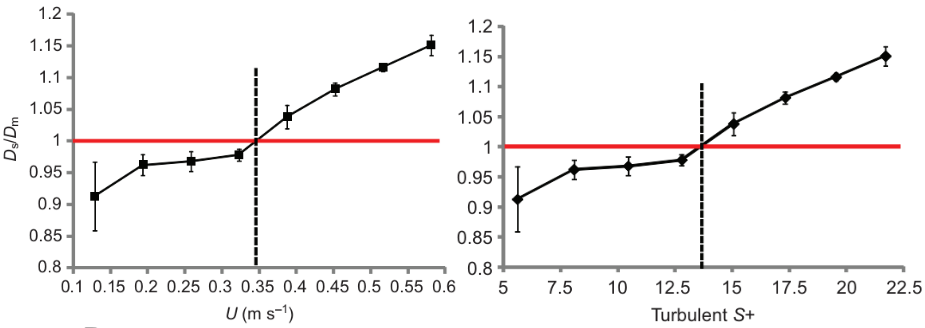
\includegraphics[width=15cm]{images/litReview/sharkScaleDragProfile1.png}
\caption{The drag reduction of a denticle array in terms of bulk velocity (left) and dimensionless riblet width (right). Image taken from \cite{wen2014}.}
\label{figure:literatureReview:dragProfileSharkScales}
\end{figure}
%
The experiments of \cite{fletcher2014phd} were carried out at a bulk velocity of $\sim$\SI{0.5}{m/s}. Figure \ref{figure:literatureReview:dragProfileSharkScales} suggests that the drag reducing cases of \cite{fletcher2014phd} should be increasing drag by $\sim$\SI{15}{\%} if the scales behave like those of \cite{wen2014}. It is interesting to note the profiles of Figure \ref{figure:literatureReview:dragProfileSharkScales} when compared to those of the riblets in Figure \ref{figure:literatureReview:ribletPerformanceRegions}; if the results of \cite{wen2014} are accurate then the viscous region observed for engineered riblets do not apply to shark scales. Two questions arise from this; how does the drag reduction behave as the riblet spacing reduces further? And is there perhaps a more appropriate length scale other than the riblet spacing? Figure \ref{figure:litReview:makoScaleWen} highlights the key dimensions of the mako scale used by \cite{wen2014}.
%
\begin{figure}[!b]
	\begin{minipage}{0.5\linewidth}
	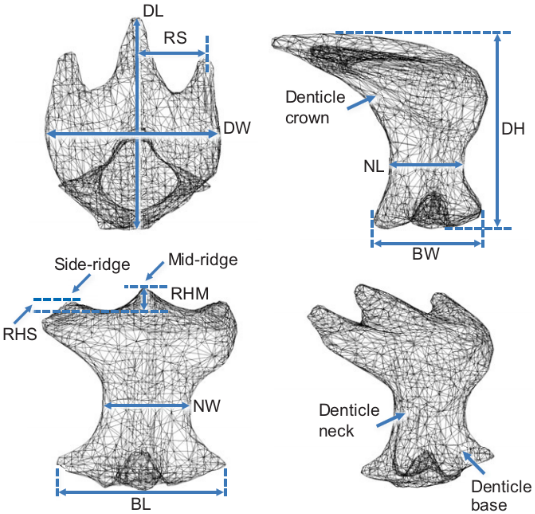
\includegraphics[width=\linewidth]{images/litReview/makoScaleOfWen.png}
	\end{minipage}
%
	\begin{minipage}{0.5\linewidth}
	\begin{tabular}{l l r}
	\hline
	Label &  & Dimension 		\\
	\hline
	\small DL, &denticle length						& \SI{151}{\mu m}	\\
	\small DW, &denticle width						&\SI{125}{\mu m}	\\
	\small DH, &denticle height						& \SI{113}{\mu m}	\\
	\small NL, &neck length							& \SI{45.1}{\mu m}	\\
	\small BW, &base width							& \SI{119}{\mu m}\\
	\small BL, &base length							& \SI{83.8}{\mu m}	\\
	\small RS, &riblet spacing						&	\SI{51}{\mu m}	\\
	\small RHM, &riblet height (mid)				&	\SI{21}{\mu m}	\\
	\small RHS, &riblet height (side)				&	\SI{11}{\mu m}	\\
	\hline	
	\end{tabular}
	\end{minipage}
\caption{Micro-CT surface mesh of a mako denticle (prior to smoothing and scaling) (left) with corresponding dimensions (right). Image taken from \cite{wen2014}.}
\label{figure:litReview:makoScaleWen}
\end{figure}
%
Clearly there are many other length scales that quantify a shark scale. The results of \cite{wen2014} are further supported by \cite{wen2015} when investigating the effects of denticle arrangements. Closely interlocked/overlapping scales are found to behave in the way indicated by Figure \ref{figure:literatureReview:dragProfileSharkScales}. In contrast, loosely interlocking scales reduce drag for $s^+ \approx 16$ by \SI{3}{\%} but increase drag for all over riblet spacings. It would be expected that the optimal riblet spacing for engineered riblets and shark scales would coincide for tightly interlocking scales but these results suggest otherwise. A major limitation noted by \cite{wen2014} is the pump range of the flume which was unable to operate below a bulk flow velocity of $\sim$\SI{0.13}{m/s}. This was also the cause of the large error bars observed in Figure \ref{figure:literatureReview:dragProfileSharkScales}. The experiments of \cite{bechert1985} determined an increased drag, for both mako and silky shark scales, for the full range of $s^+$ values. However, they did not produce results for $s^+<10$ which further supports the argument that smaller denticle riblet spacings need further investigation.

The other extreme result of Table \ref{table:litReview:denticleExperiments} is the DNS of \cite{boomsma2016}. This work adopts an immersed boundary technique to model the flow around the same denticles (staggered and aligned) printed by \cite{wen2014,wen2015}, and some engineered riblets. Periodic boundary conditions are adopted to simulate a fully developed channel flow at a Reynolds number of $Re_\tau = 180$ and a riblet spacing of $s^+=16$ (for both the engineered riblets and the denticles). The riblet surface behaved as expected; a drag reduction of $\sim$\SI{5}{\%} was predicted, arising from the reduction of the Reynolds stresses. In contrast, the denticles were found to induce separation and large vortices near the scale surface; both of which contributing to increased Reynolds stresses. The results are validated against those of \cite{bechert1985} but over predict the drag compared to \cite{wen2014,wen2015}, despite the shark scales being identical. \cite{boomsma2016} argue that this is due to the different experimental conditions of \cite{wen2014} and \cite{bechert1985}.

Referring to Table \ref{table:litReview:denticleExperiments} there is still a large spread of drag reduction results, even when ignoring the two extremes. %(why ignoring Fletcher?)
Generally the maximum drag reduction of shark scales is of a greater magnitude than those of engineered riblets, contrary to the results of \cite{bechert1985}. \cite{chen2014} observes similar drag reduction behaviour for both engineered riblets and ribletted denticles.
The denticles consistently outperformed the riblets for the full range of flow rates, achieving a maximum reduction of \SI{12}{\%}. However, there is no effort made to relate the bulk velocity to a dimensionless parameter such as $s^+$. The denticles were fabricated using a mould which was created from a real shark scale surface. The authors report a replication error of only \SI{2}{\%} but there are several issues with this technique that are not discussed. Imperfections, asymmetries, and changes in denticle geometry that exist on real shark scale arrays are all captured using the moulding technique. Clearly this model is more physical, but isolating the effects of slight geometric changes between the different denticles is unrealistic using current experimental methods. To the authors knowledge, only tightly interlocking scales have been replicated using this technique \citep{zhao2012, chen2014,zhang2011b,zhang2011a,luo2015b,luo2015}. It has yet to be established whether the same methods can be applied to more loosely interlocking scales which are equally common among different shark species (see Table \ref{figure:literatureReview:scaleVariabilityFletcher}).

A similar technique is adopted by \cite{zhao2012}; a drag reduction of 18\% is achieved at the lowest velocity measured, which then reduces to a local minimum, raising to a local maximum and then reduces to its minimum value at the highest fluid velocity. This result is not discussed, and without support from other literature the validity of the experimental techniques is questionable. \cite{zhang2011b} adopts the same moulding technology on a \textit{Isurus oxyrinchus} sample. Drag reduction is compared for a ribletted surface, sharkskin replica and a sharkskin replica with non-long polymer chains attached to the surface. The polymer surface was introduced as a method to mimic the mucus excretion of sharks. Small fishes are known to rely on mucus excretion to increase burst swimming speeds; when added to a fluid this mucus can reduce drag by up to \SI{66}{\%} \citep{fletcher2014phd}. However, unlike most fishes, sharks mucus production is restricted to small areas below the denticle crowns. It is therefore often assumed that mucus excretion has a lesser effect for sharks although the topic is still poorly understood \citep{fletcher2014phd}. %why not discussing this?
\cite{zhang2011b} measures a maximum drag reduction of \SI{8}{\%} for the sharkskin replica which increases to \SI{24}{\%} when the polymer is added. In addition to this, the drag reduction effect increases with increasing flow rate, contrary to the sharkskin without polymer added to its surface. However, \cite{fletcher2014phd} suggests that mucus is excreted from pores below the scales. \cite{zhang2011b} applies the polymer coating to the whole surface which is perhaps not a physical representation of mucus excretion. 

\cite{zhang2011a} adopts numerical and experimental techniques to investigate the drag reduction of moulded shark scales, although little detail is presented explaining either of the adopted methods. The experimental results indicate a maximum drag reduction of \SI{12.8}{\%} at the slowest flow rate which then asymptotes to a value of $\sim$\SI{9}{\%}. This behaviour is similar to that of the non-polymer covered sharkskin of \cite{zhang2011b}, although the magnitude of drag reduction is consistently $\sim$\SI{3}{\%} higher. The numerical simulations adopt a finite volume method, with a $k-\epsilon$ turbulence closure, to solve the developing flow field over an array of $\sim$30 shark scales. The shark scales were micro-CT scans of those that were replicated. While the model predicts a drag reduction of the same order as the experiments they increase from \SI{7}{\%} to \SI{14}{\%} as the flow rate increases; i.e a trend opposite to the experiments. There are several potential causes, such as a lack of grid dependence, convergence, and the use of $k-\epsilon$, which is known to perform poorly in boundary layers \citep{pope2001}. However, none of these issues are discussed by \cite{zhang2011a}. Despite this these results are often used to justify the drag reduction observed in experiments \citep{zhao2012,chen2014}.

This section has so far only discussed the literature associated with shark skin applied to flat plates and channel flows. These simple flow configurations are commonly adopted due to their applicability to a wide range of engineering flows, and the repeatability of experiments. This is made clear when referring to the riblet experiments of Section \ref{section:literatureReview:Riblets}; channel flows and flat plate experiments agree more closely than when riblets are applied to aerofoils. However, the flow field around a shark is far from the idealised flow in channels. \cite{diez2015} attempts to resolve the flow around a shortfin mako shark using Computational Fluid Dynamics (CFD). The model adopts the $k-\epsilon$ turbulence closure with wall functions to reduce computing costs. In addition to this, a roughness parameter is used to account for the denticle surface. This is clearly a large simplification to the shark scale geometry but the general flow field around the shark body is captured. The coefficient of drag as a function of position is presented in Figure \ref{figure:litReview:makoSharkFlowField}.
%
\begin{figure}[!t]
\centering
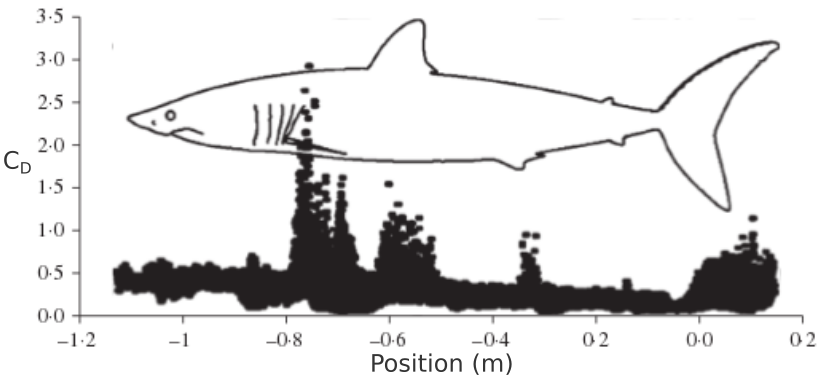
\includegraphics[width=0.8\linewidth]{images/litReview/makoSharkFlowField.png}
\caption{The coefficient of drag distribution over a mako shark. Image taken from \cite{diez2015}.}
\label{figure:litReview:makoSharkFlowField}
\end{figure}
%
 The results of \cite{diez2015} indicate a spike in the coefficient of drag near each of the fins and a slowly decreasing coefficient of drag along the main body. The authors also investigated scale morphology, whereby 24 SEM images were taken at various locations on the shark body, although little analysis is provided linking the morphology to the CFD Flow field. The authors do note that smooth scales typically exist on the leading edge of the fins and the nose of the shark. Riblets are found to be introduced further downstream. One could postulate that since a boundary layer develops from laminar to turbulent, and knowing that surface roughness has no effect in laminar flows (see Section \ref{section:literatureReview:roughness}), the transition from smooth scales to ribletted scales reflects the transition from a laminar to a turbulent boundary layer. However, the same conclusion cannot be drawn when considering the morphological study of \cite{fletcher2014phd}. Figure \ref{figure:litReview:fletcherMorphology} displays the contour maps of two denticle geometries over the body of a Lamna nasus \citep{fletcher2014phd}. 
 %
\begin{figure}[!b]
\centering
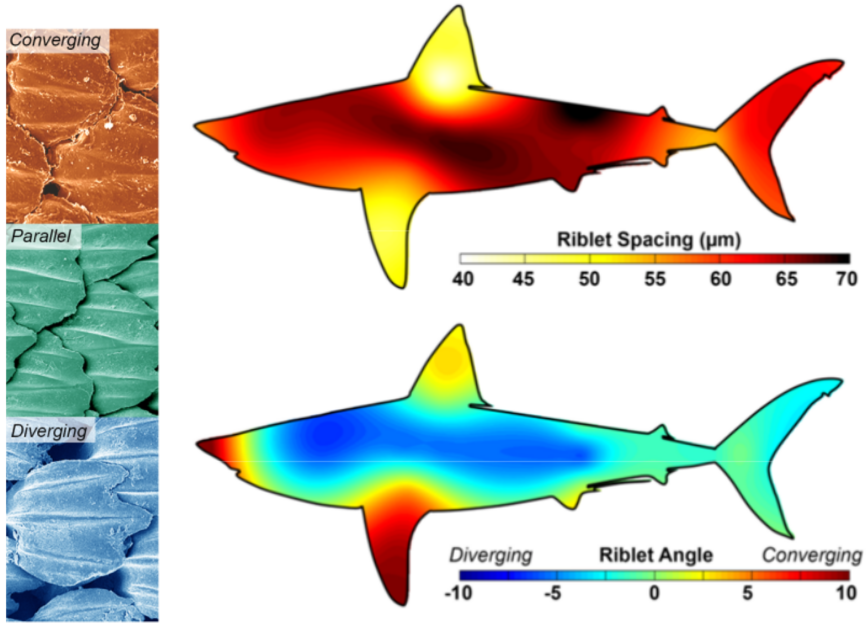
\includegraphics[width=0.8\linewidth]{images/litReview/fletcherSharkMorphology.png}
\caption{Distributions of riblet spacing and riblet angle for a Lamna nasus. Image taken from \cite{fletcher2014phd}.}
\label{figure:litReview:fletcherMorphology}
\end{figure}
%
Strongly converging riblets can be observed on the nose and pectoral fin of the fish and slightly converging scales are found on the dorsal fin. \cite{fletcher2014phd} hypothesises that converging riblets could act as a turbulent trip, similar to those observed on aerofoils (see Section \ref{section:literatureReview:Riblets}). This is further supported by the conclusions of \cite{bechert1985} who argues that denticles could increase turbulent mixing and result in a reduced susceptibility to flow separation. If this is the case then why does the mako shark analysed by \cite{diez2015} possess smooth scales on the nose? Figure \ref{figure:litReview:fletcherMorphology} also indicates reduced riblet spacing on the fins. Referring to Section \ref{section:literatureReview:Riblets} small riblet spacings are associated with higher flow rates; i.e an increase to the friction velocity, $u_\tau$ will require a reduction in riblet spacing, $s$, if the $s^+$ value is to be maintained. The findings of \cite{diez2015} reinforce this by determining an increased flow velocity near the fins of the shark. 

An aspect of shark skin that has not yet been discussed is the effect of passive bristling as a mechanism for maintaining attached boundary layers. This effect can be observed in Figure \ref{figure:litReview:bristlingScales}; while shark scales are rigid, they are embedded into a flexible epidermis which allows the denticle angle of attack to be altered \citep{lang2014}.
%
\begin{figure}[!b]
\centering
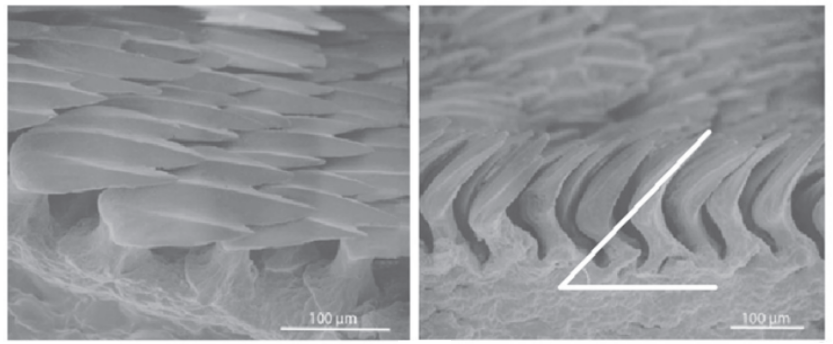
\includegraphics[width=0.8\linewidth]{images/litReview/bristlingScales.png}
\caption{Bristling scales of a shortfin mako. The scales are bristled to an angle of \SI{45}{\degree}. Image taken from \cite{lang2014}.}
\label{figure:litReview:bristlingScales}
\end{figure}
%
The precise mechanism that leads to this bristling is still unknown. \cite{bechert1985} suggested that the variation in mechanical tension of the epidermis could control the bristling mechanism. At high speeds the epidermis is under larger tension than lower speeds, and perhaps it is this mechanism that drives scale bristling. However, \cite{lang2014} concluded that the presence of recirculating flow could be enough to bristle scales alone. This is determined by imaging the effect of a small pulsating jet which created a backflow over a shark skin sample. However, the authors note that since experiments are carried out on a small section of shark skin the mechanical tension will not be matched for a real shark. \cite{lang2014} apply these sharkskin sections to a NACA 4412 aerofoil and measure the resulting flow field using Digital Particle Image Velocimetry (DPIV). They compare the resulting backflow for a sharkskin surface with bristling scales, and a smooth surface. They find that at low angles of attack the sharkskin surface produces more backflow than the smooth surface. However, backflow is substantially reduced for large angles of attack; at a foil angle of \SI{18}{\degree} there is a large amount of separation for the smooth surface but very little for the sharkskin. The authors hypothesise that at low angles of attack the backflow is too weak to induce bristling, and as a result the performance of the foil is hindered by its increased thickness. However, DPIV is unable to capture the bristling behaviour directly since the scales are so small. There are also other issues with this technique; since sharkskin is directly applied to the foil there is much uncertainty concerning the mechanical properties of the epidermis and the variability between individual scales. These issues are eliminated by the experimental technique of \cite{wen2014,wen2015} who 3D print an array of smoothed mako scales onto a flexible membrane, mimicking that of a shark epidermis. The membranes are subsequently applied to the surface of a flapping NACA aerofoil, hypothesising that the flexibility of the scales could have implications on thrust generation. Both studies conclude that the swimming speed of the self-propelling foil is increased when denticles are present but both the cost of transport (energy required per unit distance) and power required increased. The authors suggest that this is likely due to the poor representation of the flexible membrane to real shark skin where scales are more flexibly embedded into the dermis. It is suggested that dynamic experiments are more representative of shark skin and should be further investigated.

\subsection{Summary}
This section has reviewed the literature concerning engineered riblets and the experiments concerning shark scales. Several inconsistencies and gaps in the literature can be identified:
\begin{itemize}
%
\item The application of engineered riblets to flat plates and channel flows has been thoroughly investigated in the literature. However, there are still inconsistencies concerning their application to adverse and favourable pressure gradients. 
%
\item There is substantial controversy between the literature associated with the application of shark scales to flat plates and channel flows. This is due to the different experimental techniques, manufacturing methods, denticle geometries, and denticle arrangements.
%
\item While the $s^+$ scaling is appropriate for riblets, there are many denticle length scales that could also be considered; perhaps a combination of these would be more appropriate when considering the performance of denticles. 
%
\item Current experiments on denticles have been unable to investigate the effects of small values of $s^+$ on a flow. Experiments of \cite{bechert1985} and \cite{wen2014,wen2015} indicate that drag reduction occurs for denticles at a lower $s^+$ value than for engineered riblets.
%
\item Most hydrodynamic experiments have considered denticles with riblets, but there are many shark species that posses denticles without riblets. The experiments of \cite{fletcher2014phd} suggest there could be a hydrodynamic benefit to denticles without riblets. there are also many other geometrical features that have yet to be investigated, such as the effects of converging/diverging riblets on a flow. 
%
\item Some of the most informative studies concerning engineered riblets have adopted numerical methods to investigate the intricate flow fields. Numerical techniques have the advantage of being able to provide insight into how denticles interact with a flow, but only a single DNS paper has been published in this subject area. 
%
\item The application of scales to separating flows and adverse pressure gradients has seen little investigation. Studies that have been carried out in this area have focused on large scale fluid structures rather than investigating how the flow interacts with the denticles.
%
\item Dynamic experiments have also been recently introduced whereby the interactions between the flexible epidermis and the denticles are investigated. These methods can create more physical models but are currently limited to the observation of large scale structures. 
%
\item Mucus excretion is another subject that has seen little investigation in terms of shark skin. Authors have often disregarded its effect but the work of \cite{zhang2011b} suggests it could have much larger implications. 
%
\end{itemize}

\newpage

\section{Channel Flow Experiments using Laser Doppler Anemometry}
As discussed in Section \ref{section:literatureReview}, little work has been carried out in analysing the fluid flow around shark scale surfaces; most work has focussed on the use of force balances which cannot measure velocity or pressure fields. While previous experiments have successfully measured drag reduction for sharkskin they have not yet investigated the fluid dynamic features that are causing it. For this reason we choose to adopt Laser Doppler Anemometry (LDA) to measure a channel flow, with and without shark scales. While a channel flow does not replicate the complex flow fields around a shark, it allows comparison against a wide range of empirical and numerical literature data (in the case of smooth channels), and also ensures the results are applicable to a wide range of surface flows, such as boat hulls and pipe walls. In addition to this, understanding how shark scales behave in simple and controllable configurations will provide comparative data when investigating their effects on separating flows. This simplification also allows numerical models to exploit the periodicity of shark scale surfaces, greatly reducing the required computing power for numerical methods. This section details the preliminary experiments, the aim of which is to validate the experimental method and identify changes that must be made to future designs.

\subsection{Fundamentals of LDA}
LDA is a non-intrusive method of determining a fluids velocity by measuring the Doppler shift of laser light (reference the LDA book). There are several key components which can be split into two groups; an optical unit and a receiving unit. The optical unit generates and transmits a pair of laser beams for each velocity component and focusses them onto a small volume, with a typical width of \SI{100}{\mu m} (Reference). The two beams create a fringe pattern in the measurement volume, the spacing of which, $\Delta x$, is determined by the angle of intersection, $\alpha$, and the light wavelength, $\lambda$. This is demonstrated in Figure \ref{figure:experiments:fringePattern}, whereby a particle of velocity $\vect{u}_p$ passes through the fringing pattern created by the two beams $E_a$ and $E_b$. The two beams can be represented by 
%
\begin{figure}[!b]
\centering
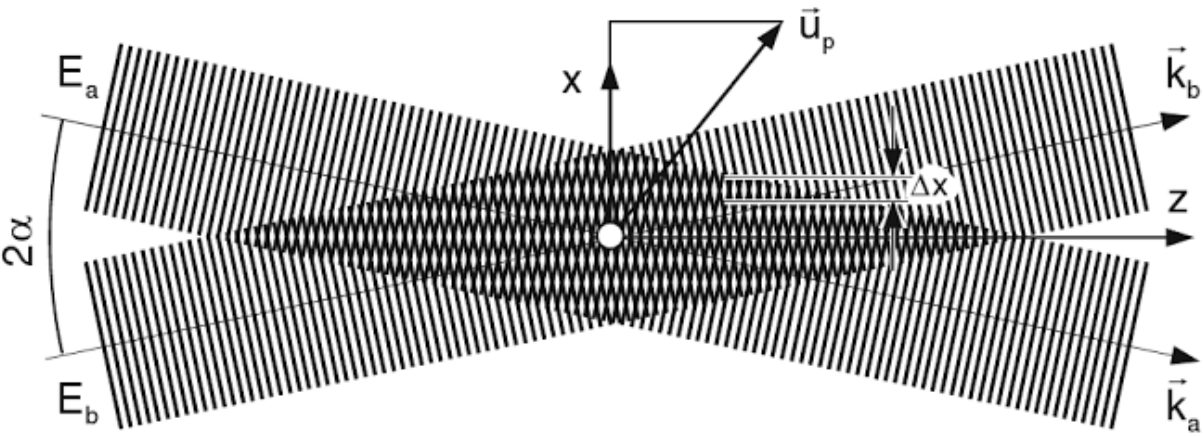
\includegraphics[width=10cm]{images/LDA_theoryImages/fringePattern.png}
\caption{Fringe pattern (LDA book reference)}
\label{figure:experiments:fringePattern}
\end{figure}
%
\begin{equation}
E_a = E_0 \cos {\left[ \omega_a t - k_a (z \cos{\alpha} - x \sin{\alpha} ) \right]},
\end{equation}
and
\begin{equation}
E_b = E_0 \cos{ \left[ \omega_b t - k_b (z \cos{\alpha} + x \sin{\alpha} ) \right]},
\end{equation}
where $E_0$ represents the wave amplitude, $\omega = 2 \pi / T$ the respective angular frequencies and $k = 2 \pi / \lambda$ the angular wavenumber. The wavelength is related to the speed of light by $c = \lambda f$ where $c$ represents the speed of light and $f$ represents the oscillation frequency. With some manipulation the $x$-component of the particle velocity is found to be directly related to both the fringe spacing and the shift in oscillation frequency as the particle passes through the fringes (Reference LDA book). The receiving components detect this change in frequency which is subsequently converted to an electrical signal and processed. In order to relate particle velocity to fluid velocity the flow is seeded with neutrally buoyant particles of \SI{40}{\mu m} diameter and it is assumed that these particles do not deviate from the fluid streamlines. 

The present work makes use of two-component LDA, whereby two pairs of beams are transmitted perpendicular to each other and of different wave lengths; one at $\lambda = $ \SI{514.51}{nm} (green light) and $\lambda = $ \SI{488}{nm} (blue light). The respective shifts in frequency are separated by the receiving unit in order to produce two velocity components. Particle velocities are also only recorded if a shift in frequency is observed by both beam pairs, thus the covariance of the two velocities (Reynolds stresses) can be analysed. 

Velocity biasing is a phenomena that must be considered when utilising LDA. Since velocities are only sampled when particles pass through the focal volume, the subsequent time series does not have a regular sampling interval. For this reason, high velocity fluctuations are measured more often than low velocity fluctuations which results in a bias towards higher velocities when calculating statistics such as means and standard deviations. The correction method of (reference) is adopted in the present work, whereby the means and standard deviations are normalised by the amount of time a particle resides in the focal volume, $\tau$. The temporal mean of a velocity component $u$ is therefore calculated by

\begin{equation}
\mu_u = \frac{\sum^N_{i=1} u_i \tau_i}{\sum^N_{i=1} \tau_i}, 
\end{equation}
the standard deviation is calculated by
\begin{equation}
\sigma_u^2 = \frac{\sum^N_{i=1} \tau_i (u_i - \mu_u)^2}{\sum^N_{i=1} \tau_i},
\end{equation}
and the covariance between the two components of velocity is calculated by
\begin{equation}
\gamma_{u,v} = \frac{\sum^N_{i=1} \tau_i (u_i - \mu_u)(v_i - \mu_v)}{\sum^N_{i=1} \tau_i}.
\end{equation}



\subsection{Experimental set up}
\label{section:experiments:setUp}
The experiments are carried out using a flat plate submerged in a recirculating flume (observed in Figure \ref{figure:experiments:setUp}).
%
\begin{figure}[!b]
\centering
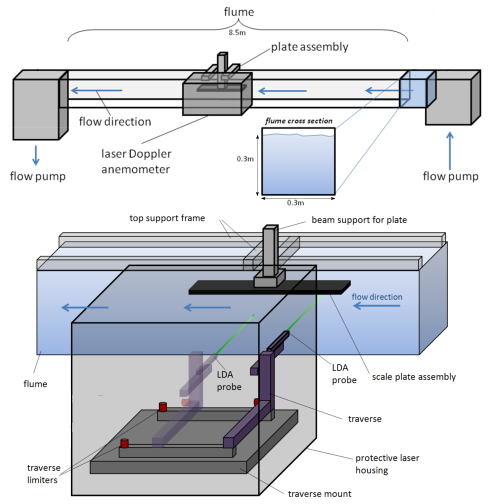
\includegraphics[width = 12cm]{images/LDA_theoryImages/expSetUp.png}
\caption{Rig design adapted from \cite{fletcher2014phd}}
\label{figure:experiments:setUp}
\end{figure}
%
The plate has the dimensions $L \times w \times h = 500 \times 100 \times 10 $ (mm) with semi-circular leading and trailing edge cross sections. The volumetric flow rate is controlled by setting the pump frequency. Relating this to a Reynolds number prior to experiments is non-trivial due to the unknown bulk velocity in-between the plate and the flume wall. Subsequently the Reynolds number is estimated from the measured profiles. The operating range of the pump is \SI{4}{Hz} to \SI{16}{Hz}. As discussed in Section \ref{section:literatureReview:sharkScaleFluids}, previous experiments have been unable to capture the effects of sharkskin at small values of $s^+$. Experiments are therefore carried out at low pump frequencies of \SI{4}{Hz} and \SI{8}{Hz}. A grid is created in order to define the locations at which the velocity is measured. The LDA probe is mounted to a traverse and calibrated such that $(0,0,0)$ lies along the centre of the plate at the most upstream point of the flat section. As discussed in Section \ref{section:literatureReview}, the viscous sub-layer exists up to $y^+ \approx 5$. If this is to be measured accurately the wall-normal grid size must be of the same order as the viscous length scale, $\delta_\nu = u_\tau / \nu$. In addition to this, the location of the wall must be known to the same order. For this reason the wall-normal zero position is set to lie in the flat plate such that the first few wall-normal grid points lie in the wall. This ensures that the full velocity profile can be captured.
% The probe is then traversed normal to the wall with a grid spacing of \SI{0.1}{mm}. For a Reynolds number of $Re_\tau \approx 400$ this equates to a spacing of $\Delta \approx 0.33 \delta_v$.
 The following grid is defined such that a high spatial resolution is present near the wall which blends into a low resolution in the far field:
\begin{align*}
\Delta = 
\begin{cases}
0.025, \hspace{1cm} &\text{for } 0 \leqslant z < 2.5,\\
0.05, \hspace{1cm} &\text{for } 2.5 \leqslant z < 3,\\
0.1, \hspace{1cm} &\text{for } 3 \leqslant z < 5,\\
0.5, \hspace{1cm} &\text{for } 5 \leqslant z < 20,\\
1, \hspace{1cm} &\text{for } 20 \leqslant z < 30,\\
5, \hspace{1cm} &\text{for } 30 \leqslant z < 75,
\end{cases}
\end{align*}
where the grid spacing, $\Delta$, and the wall-normal coordinate, $z$, are defined in \SI{}{mm}. The total number of grid points is 180 which is more than required to capture the profiles accurately. Future experiments will re-evaluate the grid based on the findings of the present study.

The time series measured at each point is passed through a moving average filter in order to remove anomalies. Anomalies are identified if they lie outside the range
\begin{equation}
\mu_{u,2s} - 2 \sigma_{u,2s} < u_{2s} < \mu_{u,2s} + 2 \sigma_{u,2s},
\end{equation}
where $s$ is half the width of the filter window. $\mu_{u,2s}$ and $\sigma_{u,2s}$ are defined by 
\begin{equation}
\mu_{u,2s} = \frac{\sum^s_{i=-s} u_i \tau_i}{\sum^s_{i=-s} \tau_i}, 
\end{equation}
and,
\begin{equation}
\sigma_{u,2s}^2 = \frac{\sum^s_{i=-s} \tau_i (u_i - \mu_{u,2s})^2}{\sum^s_{i=-s} \tau_i}.
\end{equation}
The anomalies identified by the filter were removed from the data set rather than replaced. Other filters were also tested; a global averaging method was found to remove 'real' data due to its inability to differentiate between anomalies and low/high speed structures passing through the probe volume. The filtering method of \cite{goring2002}, designed for Acoustic Doppler Anemometry data, was also found to identify more anomalies than expected. 


%			NOTE - Y+ VALUES ARE DIFFERENT FOR DIFF FLOW RATES


%!!!!	The mechanism controlling vortex shedding from rectangular bluff bodies !!! - This paper suggests a St number of 1 and therefore a shedding frequency of roughly 5/4. 


\subsection{Preliminary Results}
Two sets of results are presented in this section; a time dependence analysis of the means, standard deviations, and the covariance of the two velocity components; and an analysis of the measured profiles. The time dependence study investigates the convergence of statistics as a function of the averaging time. This allows the errors associated with short averaging windows to be estimated, and also provides information regarding how much averaging time is required to reduce the error to an acceptable level. The second section investigates the spatial dependency on the flow statistics which will ultimately be used to compare the differences between sharkskin and smooth surfaces.
% The preliminary results will provide an estimate to the possible Reynolds number range, the coefficient of skin friction, and the development of the boundary layer over the plate. 

\subsubsection{Time Dependence}
\label{section:experiments:timeDep}

Time dependence was assessed at three vertical locations, \SI{400}{mm} from the upstream end of the plate. These positions were at $z=$\SI{1}{mm}, \SI{15}{mm}, and \SI{40}{mm}. It was assumed that these locations would provide enough data to predict the error associated with the choice of sampling time. Several positions are chosen since the amount of sampling time required is dependent on the local velocity of the flow. It is therefore expected that close to the wall, statistics will require a longer averaging window. This analysis also investigates how the statistics converge against the number of samples measured. This is dependent on the sampling rate of the LDA, and the local time scale of the flow. It is expected that high local velocities will result in a higher sampling rate.

 The probe measured velocities for \SI{300}{s} at each location for pump speeds of \SI{4}{Hz} and \SI{8}{Hz}. The mean streamwise velocity as a function of time is defined as $\mu_u (t) = \mu_u[0,t]$. The standard deviations and covariance are defined using the same notation. Convergence is determined by normalising these quantities against their evaluation over the whole time series. These reference values can be observed in Table \ref{table:experiments:convergedStatistics}.
 %
 \begin{table}[!h]
 \centering
 \caption{...}
 \label{table:experiments:convergedStatistics}
 \begin{tabular}{c c c c c c c}
 \hline
 Pump Frequency	&	$z$ location	&	$\mu_u(300)$	&	$\mu_v(300)$	&	$\sigma_u(300)$	&	$\sigma_v(300)$	&	$\gamma_{u,v}(300)$	\\
 %
 \multicolumn{1}{c}{(\SI{}{Hz})}	&	\multicolumn{1}{c}{(\SI{}{mm})}	&	\multicolumn{1}{c}{(\SI{}{m/s})}	&	\multicolumn{1}{c}{(\SI{}{m/s})}	&	\multicolumn{1}{c}{(\SI{}{m/s})}	& \multicolumn{1}{c}{(\SI{}{m/s})}	& \multicolumn{1}{c}{(\SI{}{m^2/s^2})}	\\
%
\hline
4	&	1	&	0.027081	&	-0.000173	&	0.008319	&	0.000773	&	-0.000002	\\
4	&	15	&	0.091392	&	-0.000447	&	0.008947	&	0.005598	&	-0.000019	\\
4	&	40	&	0.100255	&	-0.000787	&	0.008099	&	0.005211	&	-0.000011	\\
8	&	1	&	0.085152	&	-0.000843	&	0.023807	&	0.003023	&	-0.000031	\\
8	&	15	&	0.185502	&	-0.001367	&	0.015663	&	0.009869	&	-0.000047	\\
8	&	40	&	0.204352	&	-0.001552	&	0.013103	&	0.008496	&	-0.000027	\\
\hline
 
 \end{tabular}
 \end{table}
 %

Figures \ref{figure:experiments:timeDependence:meanUx} to \ref{figure:experiments:timeDependence:uv} indicate how the statistics converge as the averaging time, and sample number, increase. For clarity, only the two extreme $z$ positions are plotted. Figure  \ref{figure:experiments:timeDependence:meanUx} indicates fast convergence for the mean streamwise velocity at $z=$\SI{40}{mm} for both pump speeds.
%
\begin{figure}[!h]
\centering
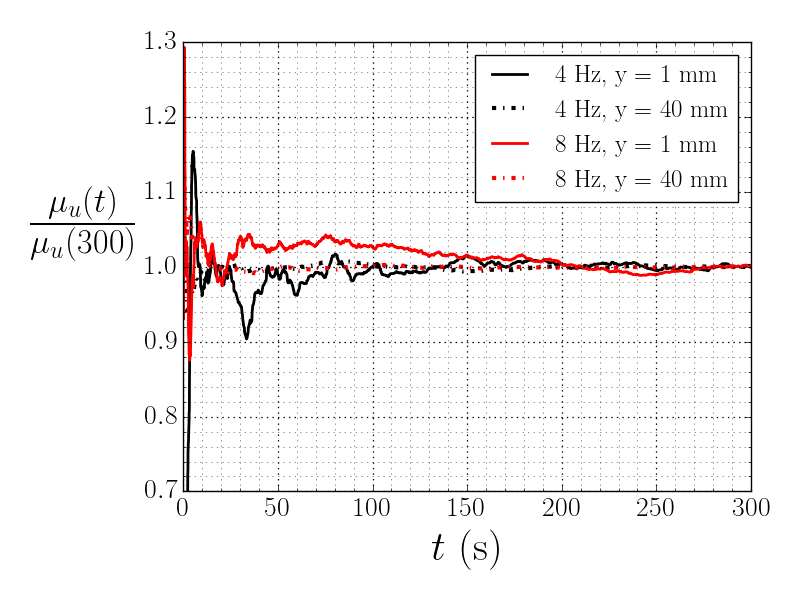
\includegraphics[width=0.5\linewidth]{images/LDA_timeDependenceImages/UxMeanTConvergence.png}\hfill
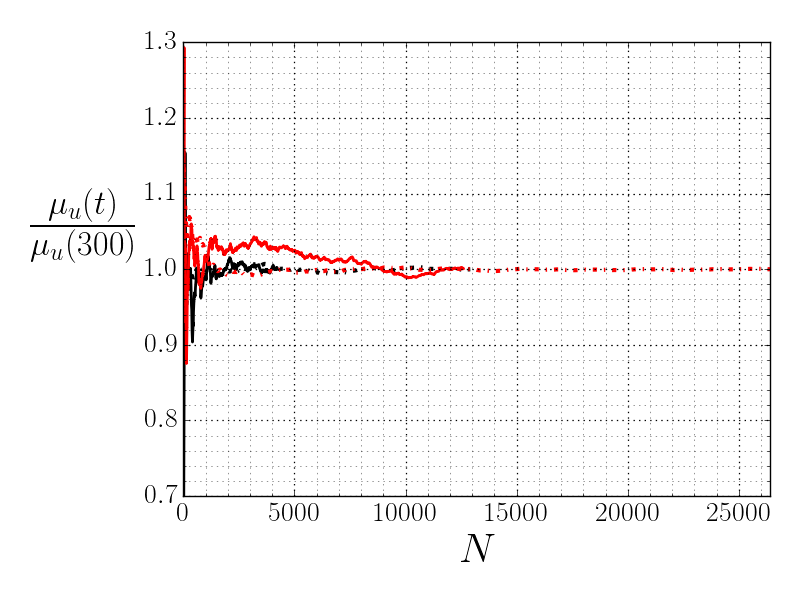
\includegraphics[width=0.5\linewidth]{images/LDA_timeDependenceImages/UxMeanNConvergence.png}\\
\caption{Convergence of the mean streamwise velocity as a function of time (left) and sample number (right).}
\label{figure:experiments:timeDependence:meanUx}
\end{figure}
%
 An averaging window of $\lesssim$ \SI{30}{s} can reduce the error to below \SI{1}{\%}. As expected, the mean streamwise velocity converges more slowly near the wall. After $\sim$\SI{30}{s} convergence to $\sim$\SI{5}{\%} is achieved for the pump frequency of \SI{8}{Hz} but only \SI{10}{\%} for \SI{4}{Hz}. In order to reduce the low pump frequency error to below \SI{5}{\%} an averaging window of $\sim$\SI{50}{s} is required. Both pump frequencies require an averaging window of $\sim$\SI{200}{s} to converge to within a $\sim$\SI{1}{\%} error. In terms of the number of samples, it takes more than twice as many to converge for the higher pump frequency. These results suggest that convergence of the mean streamwise velocity is more dependent on averaging time rather than the number of samples obtained. 
 
Figure \ref{figure:experiments:timeDependence:meanUy} indicates very poor convergence for the mean vertical component of velocity, especially for the low pump frequency.
%
\begin{figure}[!h]
\centering
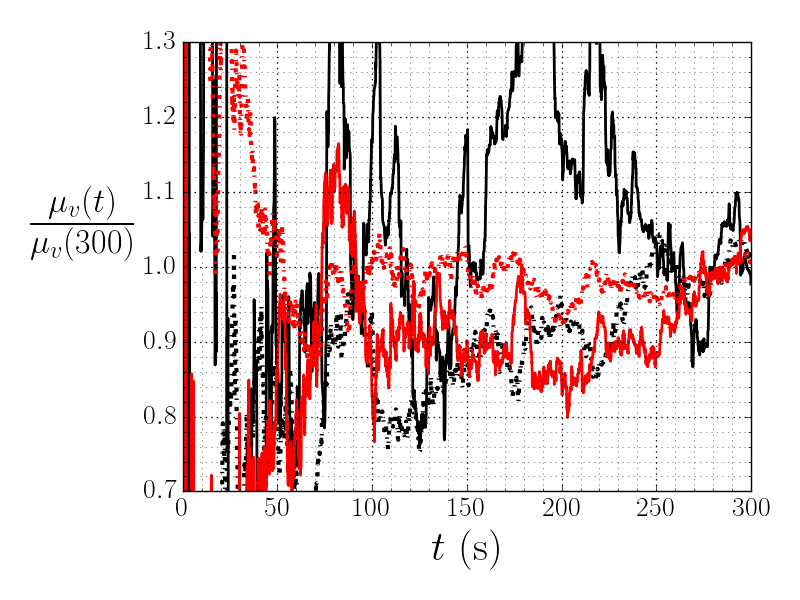
\includegraphics[width=0.5\linewidth]{images/LDA_timeDependenceImages/UyMeanTConvergence.png}\hfill
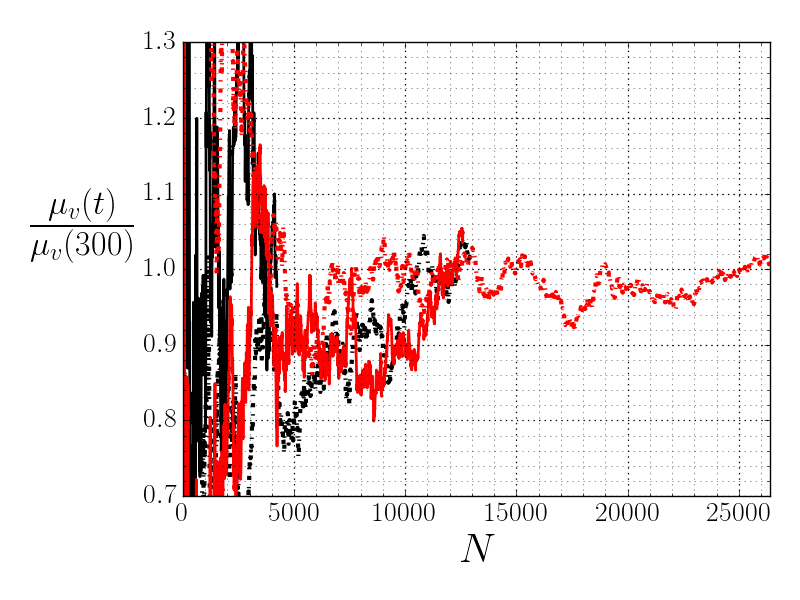
\includegraphics[width=0.5\linewidth]{images/LDA_timeDependenceImages/UyMeanNConvergence.png}\\
\caption{Convergence of the mean wall-normal velocity as a function of time (left) and sample number (right). For legend, see Figure \ref{figure:experiments:timeDependence:meanUx}.}
\label{figure:experiments:timeDependence:meanUy}
\end{figure}
%
 This is likely due to the tolerances of the LDA; the recorded wall-normal velocities are of the order  \SI{0.1}{mm/s} for the low pump frequency. This is at least two orders of magnitude lower than the streamwise velocity measurements, even close to the wall. For completeness the statistics were not omitted, but the mean wall-normal velocity is rarely published in boundary layer literature. 

The standard deviations are important due to their relationship with the turbulent kinetic energy and the Reynolds stresses. As observed in Figure \ref{figure:experiments:timeDependence:RMSux}, the standard deviations of the streamwise velocity, at a pump frequency of \SI{4}{Hz}, converge at the same rate for both vertical positions, taking $\sim$\SI{130}{s} to reduce to a \SI{5}{\%} error, and $\sim$\SI{200}{s} to reduce to \SI{2}{\%}. 
%
\begin{figure}[!h]
\centering
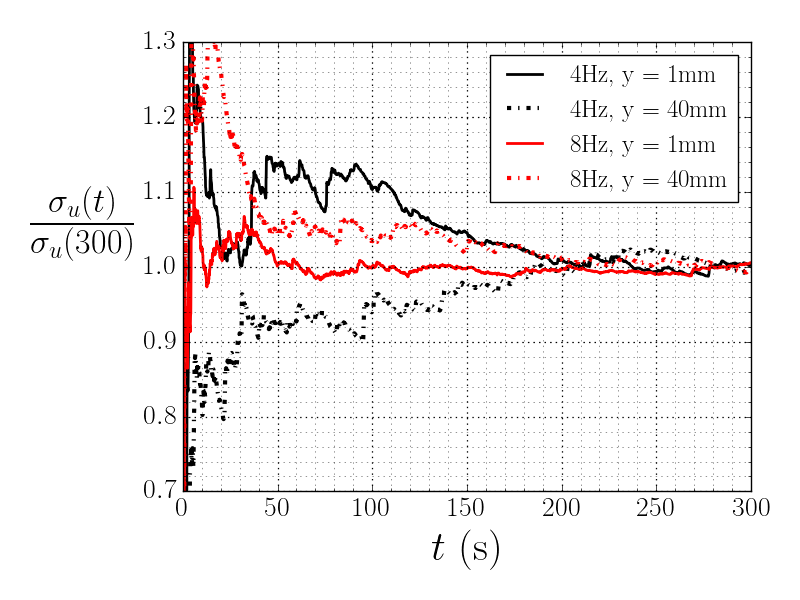
\includegraphics[width=0.5\linewidth]{images/LDA_timeDependenceImages/uxRMSTConvergence.png}\hfill
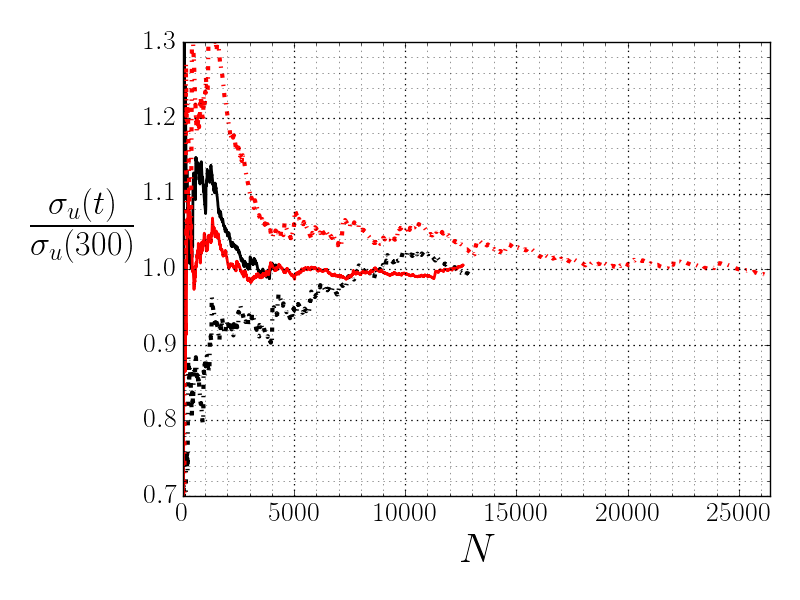
\includegraphics[width=0.5\linewidth]{images/LDA_timeDependenceImages/uxRMSNConvergence.png}\\
\caption{Convergence of the standard deviation of the streamwise velocity as a function of time (left) and sample number (right). For legend, see Figure \ref{figure:experiments:timeDependence:meanUx}.}
\label{figure:experiments:timeDependence:RMSux}
\end{figure}
%
In contrast, the standard deviation at $z=$\SI{1}{mm} converges more quickly than at $z=$\SI{40}{mm}, for the higher pump frequency. This can be explained by referring to Table \ref{table:experiments:convergedStatistics}; for a pump frequency of \SI{4}{Hz} the magnitude of $\sigma_u$ is of a similar magnitude for both $z$ locations. This is not the case for the higher pump frequency; at $z=$\SI{1}{mm} the magnitude of $\sigma_u$ is larger than at $z=$\SI{40}{mm}, suggesting that convergence is related to the magnitude of the statistic in question. At $z=$\SI{1}{mm} the standard deviation reduces to an error of $\sim$\SI{2}{\%} after just \SI{60}{s}. In contrast, it takes $\sim$\SI{200}{s} at $z=$\SI{40}{mm}. Figure \ref{figure:experiments:timeDependence:RMSux} also indicates that convergence is more dependent on the averaging time rather than the number of samples. After $\sim$\SI{200}{s} all four profiles have converged within $\sim$\SI{2}{\%} of their final value, but there is no common sample number that suggests convergence. 

The convergence of the wall-normal velocity standard deviations can be observed in Figure \ref{figure:experiments:timeDependence:RMSuy}.
%
\begin{figure}[!h]
\centering
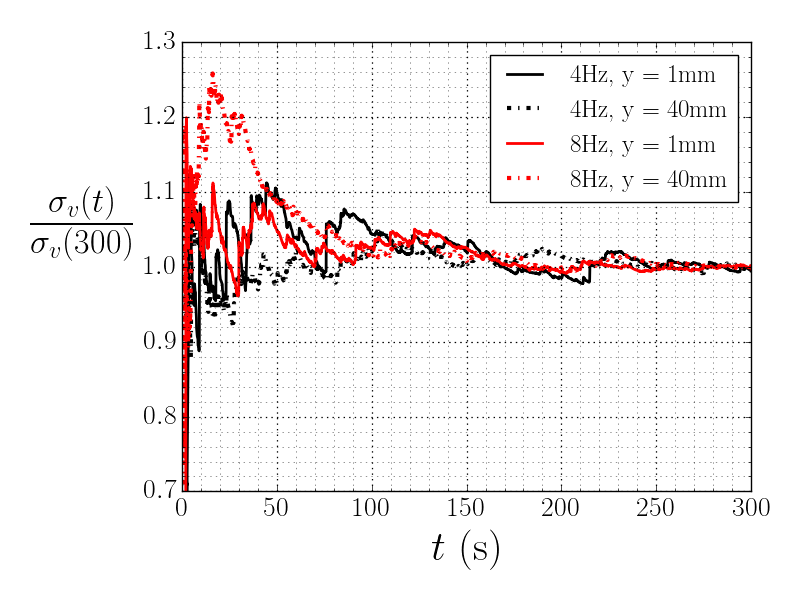
\includegraphics[width=0.5\linewidth]{images/LDA_timeDependenceImages/uyRMSTConvergence.png}\hfill
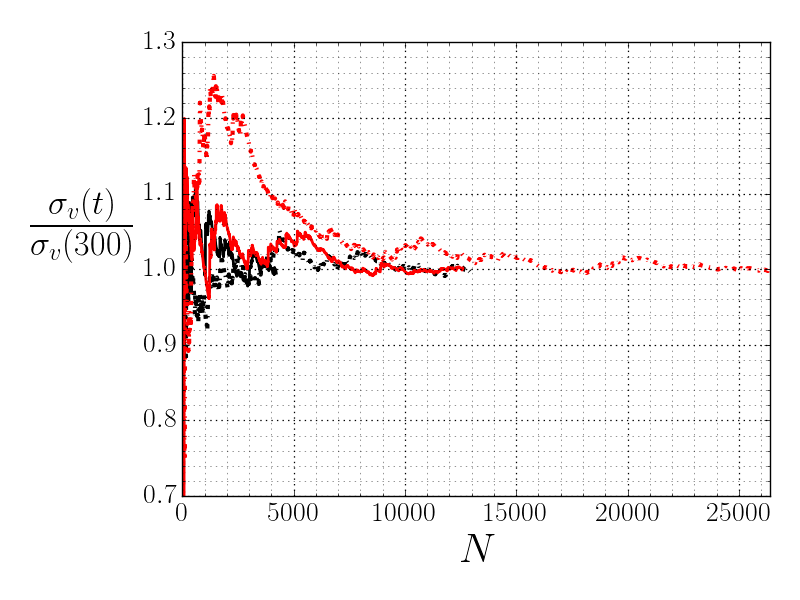
\includegraphics[width=0.5\linewidth]{images/LDA_timeDependenceImages/uyRMSNConvergence.png}\\
\caption{Convergence of the standard deviation of the wall-normal velocity as a function of time (left) and sample number (right). For legend, see Figure \ref{figure:experiments:timeDependence:meanUx}.}
\label{figure:experiments:timeDependence:RMSuy}
\end{figure}
%
After $\sim$\SI{100}{s} all four profiles converge at the same rate. An error of $\sim$\SI{4}{\%} is obtained after \SI{100}{s} and $\sim$\SI{2}{\%} after \SI{220}{s}. Again, convergence appears to be more dependent on the time interval rather than the number of samples.

The covariance of the two velocity components convergences very slowly, as indicated by Figure \ref{figure:experiments:timeDependence:uv}.
%
\begin{figure}[!h]
\centering
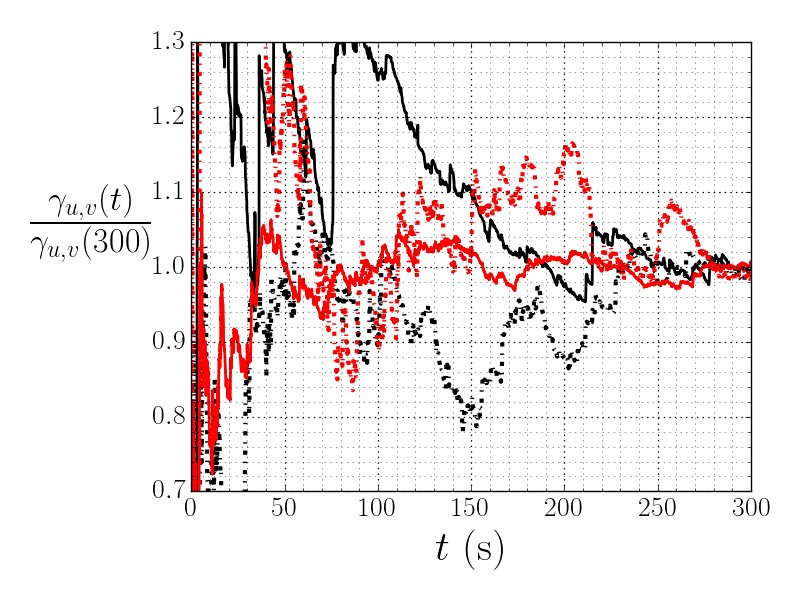
\includegraphics[width=0.5\linewidth]{images/LDA_timeDependenceImages/uvTConvergence.png}\hfill
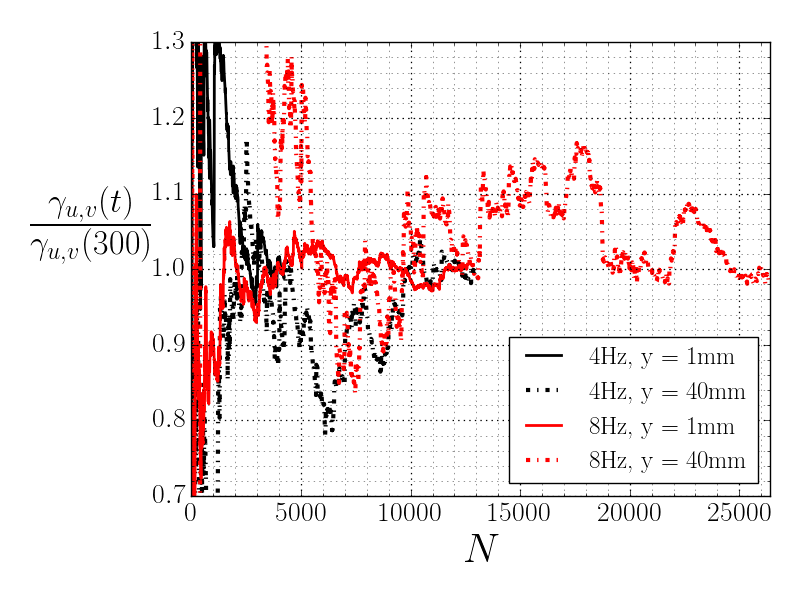
\includegraphics[width=0.5\linewidth]{images/LDA_timeDependenceImages/uvNConvergence.png}\\
\caption{Convergence of the covariance of the streamwise and wall-normal velocities as a function of time (left) and sample number (right). For legend, see Figure \ref{figure:experiments:timeDependence:meanUx}.}
\label{figure:experiments:timeDependence:uv}
\end{figure}
%
Even after \SI{300}{s}, only the near wall point for the high pump frequency indicates reasonable convergence which reduces the error to $\sim$\SI{2}{\%} after $\sim$\SI{250}{s}. Although this estimate makes the assumption that $\gamma_{u,v}(300)$ represents the 'true' value. Figure \ref{figure:experiments:timeDependence:uv} also highlights some sudden jumps in the near wall, low pump speed covariance. This could have arisen from non-physical spikes in the $(u-\mu_u)(v-\mu_v)$ time series. Perhaps the filtering method should be applied to more than just the $u$ and $v$ data sets. However, the other three covariances still predict an error of $>$\SI{10}{\%} after \SI{200}{s} of averaging time. Clearly, if the Reynolds stresses are to be used to analyse the effect of shark skin then longer averaging times will be required. 

\subsubsection{Profile plot section}
The means, standard deviations and covariance of velocity are measured along profiles at $z=$\SI{300}{mm} and $z=$\SI{400}{mm}. The vertical locations are given in the grid defined in Section \ref{section:experiments:setUp} and profiles are measured for a pump frequency of \SI{4}{Hz} and \SI{8}{Hz}. Due to time constraints, velocities were only sampled for \SI{20}{s}. The errors associated with this are estimated by using the time dependence analysis of Section \ref{section:experiments:timeDep}; for a statistic $\phi$, such as the mean streamwise velocity, the error is estimated by
\begin{equation}
\label{equation:experiments:errorCalc}
e_\phi = \mathbf{E} \left( \mid
				\phi(300) - \phi[t-10,t+10]
					\mid \right), \hspace{1cm} \text{for } 10 \leq t \leq 290.
\end{equation}
This method sweeps through the entire length of the \SI{300}{s} time series and calculates the error between the \SI{20}{s} estimated statistic, $\phi[t-10,t+10]$, and its `true' value, $\phi(300)$. The expectation of the magnitude of this quantity is taken as the error. However, since the error can only be estimated at three veritcal locations we must interpolate to fit the entire profile. Future work will consider many more locations to estimate this error. 

The mean streamwise velocity profiles can be observed in Figure \ref{figure:experiments:profiles:meanU}.
%
\begin{figure}[!h]
\centering
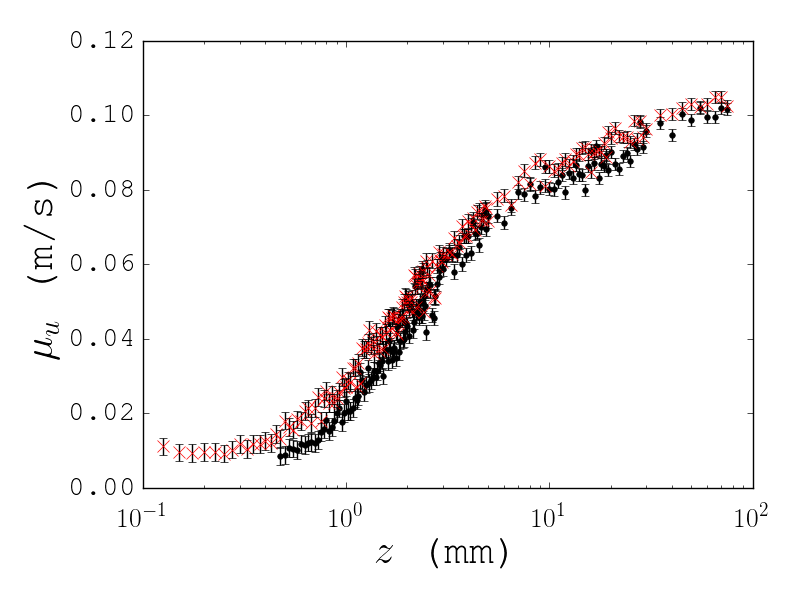
\includegraphics[width=0.5\linewidth]{images/LDA_profileImages/meanU_4hz.png}\hfill
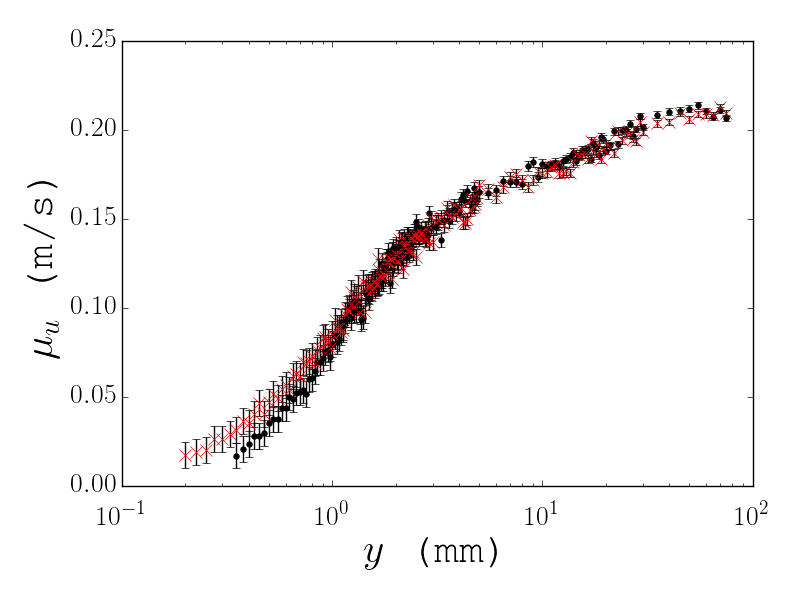
\includegraphics[width=0.5\linewidth]{images/LDA_profileImages/meanU_8hz.png}
\caption{Raw profiles of mean streamwise velocity for pump frequencies of \SI{4}{Hz} (left), and \SI{8}{Hz} (right). Symbols represent the following: $\color{black}{\bullet}$, $\mu_u$ at $x=$ \SI{300}{mm}; $\color{red}{\times}$, $\mu_u$ at $x=$ \SI{400}{mm}.}
\label{figure:experiments:profiles:meanU}
\end{figure}
%
 The logarithmic region of the \SI{8}{Hz} pump frequency can be distinguished as the linear trend between $\sim$\SI{2}{mm} and $\sim$\SI{20}{mm} but it is harder to locate for the low pump frequency. This is due to its shorter length and a larger spread in the data, likely due to the short averaging time. However, the viscous and buffer regions are especially well resolved for the mean velocity. Figure \ref{figure:experiments:profiles:meanU} also shows a collapse of the $z=$ \SI{300}{mm} and $z=$ \SI{400}{mm} for the higher flow rate, with a small deviation near the wall. This suggests that the velocity profiles are close to fully developed. In contrast, the lower frequency flows indicate a slightly reduced velocity for the entire measured profile. It should be noted that the profiles were only measured up to \SI{75}{mm} due to experimental constraints. Future experiments will be revised such that half the height of the channel can be measured (\SI{10}{mm}). The low pump frequency results also indicate more points captured in the downstream profile. This suggests that the plate is not quite flat. However, a difference in \SI{0.4}{mm} over a distance of \SI{100}{mm} equates to an angle of $\sim$\SI{0.3}{\degree} and can therefore be neglected. 
 
The standard deviation profiles can be observed in Figure \ref{figure:experiments:profiles:std}.
%
\begin{figure}[!h]
\centering
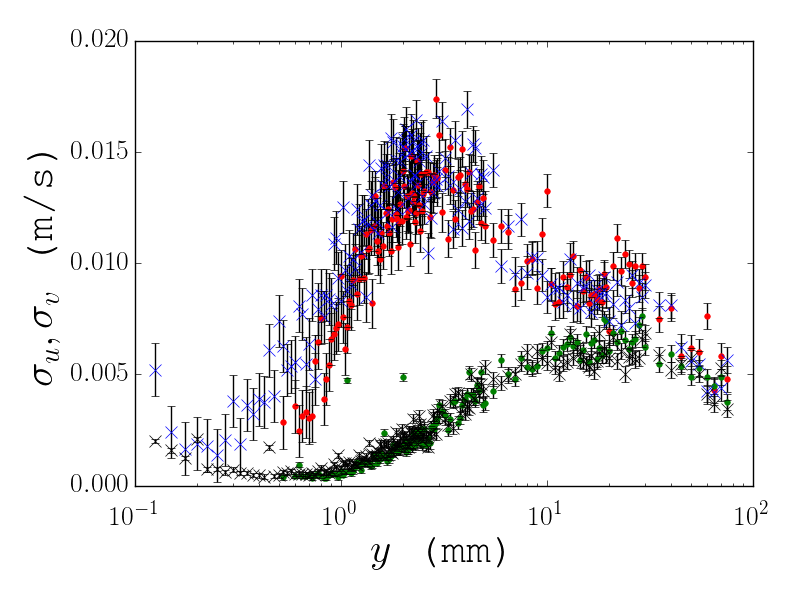
\includegraphics[width=0.5\linewidth]{images/LDA_profileImages/std_4hz.png}\hfill
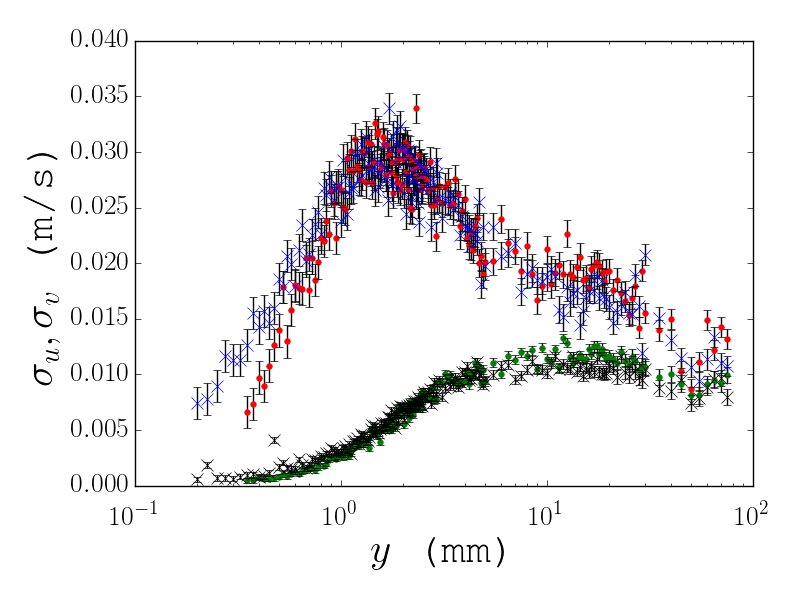
\includegraphics[width=0.5\linewidth]{images/LDA_profileImages/std_8hz.png}
\caption{Raw profiles of standard deviations of velocity for pump frequencies of \SI{4}{Hz} (left), and \SI{8}{Hz} (right). Symbols represent the following: $\color{red}{\bullet}$, $\sigma_u$ at $x=$ \SI{300}{mm}; $\color{blue} \times $, $\sigma_u$ at $x=$ \SI{400}{mm}; $\color{green}{\bullet}$, $\sigma_v$ at $x=$ \SI{300}{mm}; $\color{black} \times $, $\sigma_v$ at $x=$ \SI{400}{mm}.}
\label{figure:experiments:profiles:std}
\end{figure}
%
The wall-normal fluctuations are captured reasonably well for both pump speeds. The two $z$ locations collapse until $z\approx$ \SI{1}{mm}, at which point the wall-normal standard deviations reach their maximum and a larger spread of the data can be observed. At a pump frequency of \SI{8}{Hz} the streamwise fluctuations reach a maximum in the buffer region. There is a lot of spread in the data, clearly suggesting that longer averaging times are required. Despite the spread in data, a collapse can be observed in the buffer layer, between the two $z$ profiles. These differentiate nearer the wall, indicating that the fluctuations are of a greater magnitude further along the plate. The \SI{4}{Hz} standard deviations indicate a much larger error in the streamwise direction.  The plot also indicates that there is much more spatial resolution between $z=$ \SI{1}{mm} and $z=$\SI{3}{mm} than is required. 

The profiles of velocity covariance can be observed in Figure \ref{figure:experiments:profiles:gamma}.
%
\begin{figure}[!h]
\centering
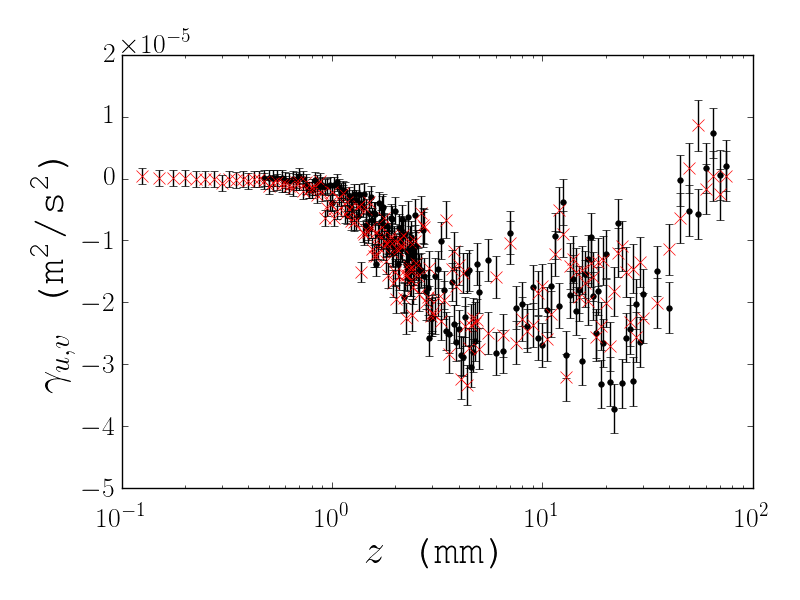
\includegraphics[width=0.5\linewidth]{images/LDA_profileImages/cov_4hz.png}\hfill
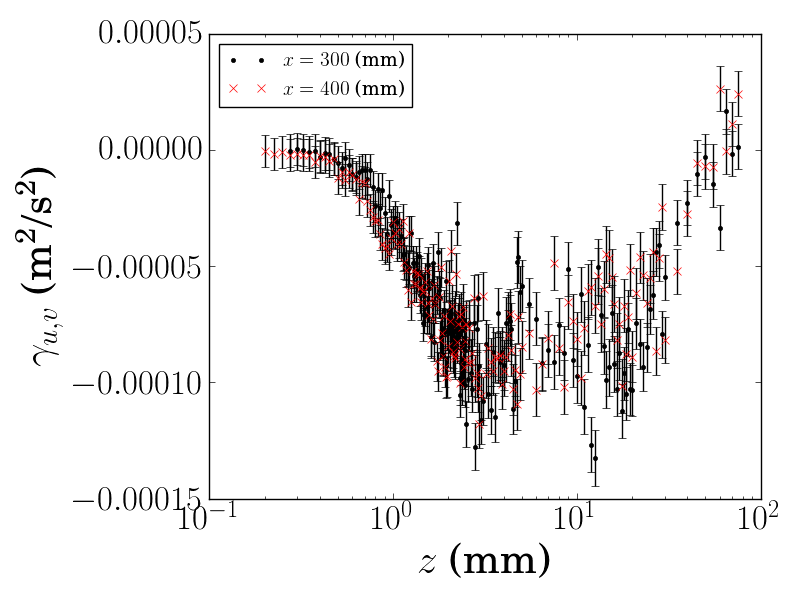
\includegraphics[width=0.5\linewidth]{images/LDA_profileImages/cov_8hz.png}
\caption{Raw profiles of the covariance of the two velocity components for pump frequencies of \SI{4}{Hz} (left), and \SI{8}{Hz} (right). Symbols represent the following: $\color{black}{\bullet}$, $\gamma_{u,v}$ at $x=$\SI{300}{mm}; $\color{red}{\times}$, $\gamma_{u,v}$ at $x=$\SI{400}{mm}.}
\label{figure:experiments:profiles:gamma}
\end{figure}
%
The covariance indicates a large spread in the data as the distance from the wall increases. The estimated error bars do reflect this increase in uncertainty but the magnitude seems too small in this case. This is likely due to the lack of points used to estimate these errors. It could also be due to the fluctuations in the errors which are not reflected by taking the expectation in \eqref{equation:experiments:errorCalc}. Future work will investigate the effect of taking into account the standard deviations. It is clear from Figure \ref{figure:experiments:profiles:gamma} that if the Reynolds stresses are to be compared between smooth and sharkskin surfaces then a much longer averaging time is required.

Conclusions and future work:
- we can reduce number of $Z$ points
- clearly not fully developed for slower flows
- very well resolved mean profiles
- reasonable RMS for high flow rate
- need more averaging time for lower flow rate and reynolds stresses
- future work will adopt different methods to calculating Utau in order to normalise data
- 





\newpage
\section{Work So Far ...}
A review of the literature indicates two areas that have not been adequately investigated: Analysis of the effect of scale geometry on the flow field, and the impact of scales on separating flows. Proprietary work has, so far, concentrated on the first of those areas, although the techniques adopted are transferable to the latter. A parametric study is to be carried out, in order to investigate the effects of scale geometry on the fluid flow. This tool will exploit the periodicities and symmetries associated with arrayed scales, resulting in an infinitely long and wide computational domain. For smooth walls, an extensive range of DNS data is available, making the validation of early work straight forward. The parametric tool requires several work packages to be completed before it can be used. In order to reduce computational expense, the parametric tool will adopt RANS methods. Experimental methods could be adopted to validate the RANS model, but these will only allow validation of the fields far from the scales, due to resolution issues. This will instead be combined with a high resolution LES, which will capture the flow around the scales. Progress has been made in three areas over the last 6 months:

\begin{itemize}
\itemsep0em
\item The creation of a simplified shark scale using CREO Parametric CAD software,

\item Preliminary experimentation with several meshing packages in order to select the most appropriate software,

\item and the implementation and validation of an LES channel flow.
\end{itemize}

Each of these will be discussed in the following sections.

\subsection{CAD: Replication of a shark scale}
\label{section:cad}
This Section details the process adopted to replicate and simplify a \textit{Poracanthodes sp.} fish scale (sampled by \cite{fletcher2014phd}) for fluid dynamic analysis. This particular scale was chosen due to its relatively simple geometry. Other sampled scales included other geometric features, such as riblets, which are not yet of interest. The implications of these additional features will be investigated through the parameter study. The Computer Aided Design (CAD) process, carried out using CREO Parametric software, is required in order to create an array of scales suitable for manufacture and LDA experimentation. The CAD model is also required in order to carry out numerical analysis; a body fitted mesh will be constructed using the CAD in order to adopt finite volume methods.

The scale sample, provided by \cite{fletcher2014phd}, is displayed in figure \ref{figure:scaleSample}. It can be observed from this image that there are many sharp edges that have been introduced, possibly by a lack of resolution from the scanning equipment, defects on the scale sample, or damage to the sample.
\begin{figure}[!b]
\centering
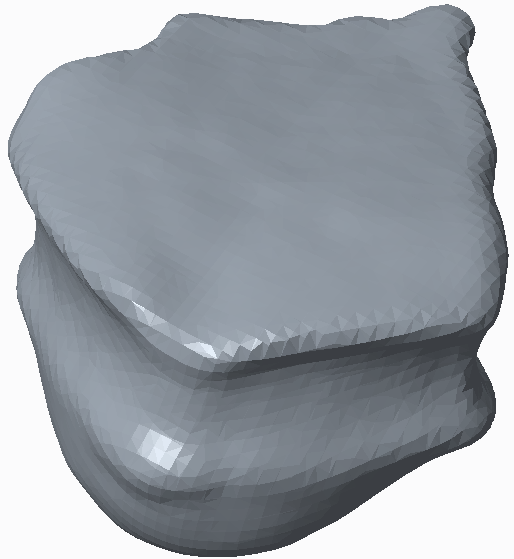
\includegraphics[width=6cm]{images/Scale_Replication_1.PNG}\hfill
\caption{\textit{Poracanthodes sp.} sample from \cite{fletcher2014phd}.}
\label{figure:scaleSample}
\end{figure}
There are also many asymmetries that exist, such as the wave-like shapes on the trailing edge of the scales. These features are likely due to the discrepancies between scale samples; even scales in tightly packed arrays are known to vary in geometry from scale to scale \citep{fletcher2014phd}. In addition to this, a large portion of the scale is embedded in the dermis of the fish and therefore has no effect on the hydrodynamics of the scale. For these reasons a simplified scale is created, based on the \textit{Poracanthodes sp.} sample. The simplified replica removes the sharp faceted features, the asymmetries and the portion of the scale that lies underneath the fish dermis.

\subsubsection{Methodology}
A coordinate system is fitted to the scale and 10 datum planes are created in the $xz$ plane with equal spacings between the first 7 and last 3 planes. The first set of planes extend to the point of maximum width of the sample and the last three are placed in order to capture the steep gradients beyond this point. A sketch is created at each of these planes resembling the cross section of the scale sample but using primitive shapes that can later be parametrised. An example of this is presented in Figure \ref{figure:crossSection};

the wave-like shapes on the downstream section of the scale has been removed and the sketch is symmetric about the central axis. This is achieved by using three arcs connected by tangential lines, reducing each section to three radius parameters, three vertical positions and a single horizontal position (as observed in Figure \ref{figure:crossSection}). Each sketch can therefore be represented by a displacement from the $y=0$ plane and 7 dimensions defining the sketch section. This makes parameter studies straight forward to implement in future work. 

\begin{figure}[!b]
\centering
\vcenteredhbox{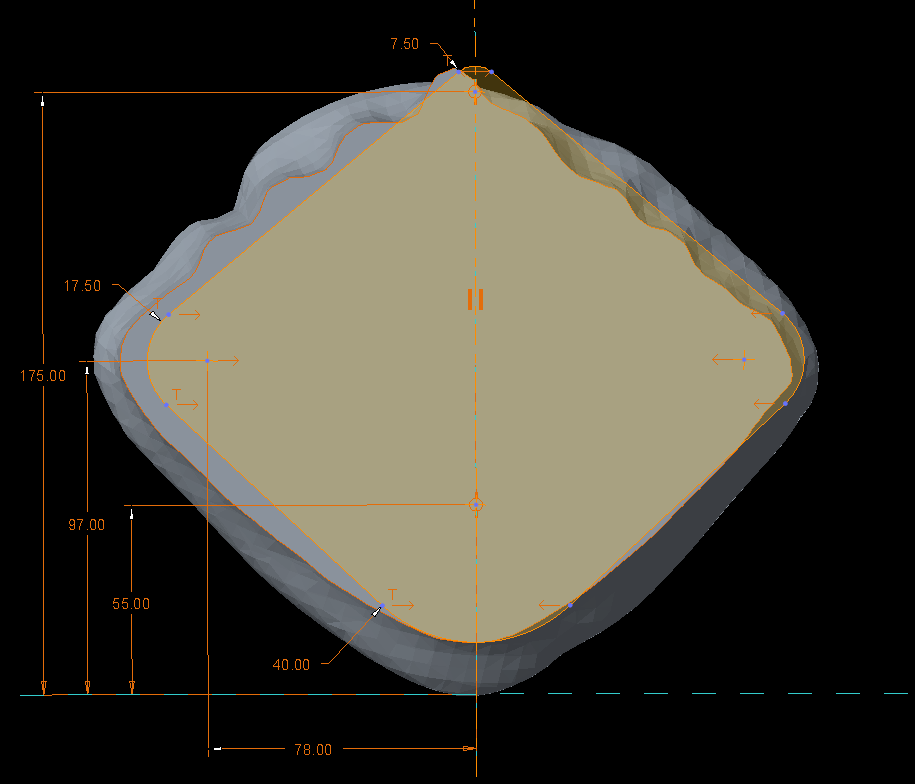
\includegraphics[width=12cm]{images/cross_section_sketch.PNG}}
\caption{A comparison between a simplified cross section and the sampled scale cross section. The dimensions are scaled after the simplified scale is generated.}
\label{figure:crossSection}
\end{figure}

The sketches are blended together using a `protrusion blend' function, creating the CAD model on the right of Figure \ref{figure:blendedScale}. An undesirable feature of this technique is that the top surface is orthogonal to the defined datum plane. In order to create a more natural curved surface a warping tool, unique to Creo Parametric, is adopted. This tool creates a mesh around the object and allows free-hand manipulation of the surface by moving the mesh nodes. This process allows an organic Scale to be created which more closely resembles that of the original sample. However, parametrising the `warping' tool is non-trivial. Further work in this area will be carried out in order to develop a more systematic approach, but for initial experimentation this `one-off' scale is appropriate.

The final scale replica is compared against the scanned sample in Figure \ref{figure:scaleComparison}. The model is scaled to a height of $H^+ \sim 10$ at a Reynolds number of $Re_\tau = 180$ for preliminary meshing experiments. This will later be scaled to a suitable size for both 3D printing, LDA experiments and a high resolution LES. The scales are arranged into a staggered array (Figure \ref{figure:staggeredArray}) with an addition two parameters to define; a spacing in $x$ and in $z$. The exploitation of this periodic arrangement, through the use of CFD, will be discussed in Section \ref{section:meshing}.

\begin{figure}[!t]
\centering
\vcenteredhbox{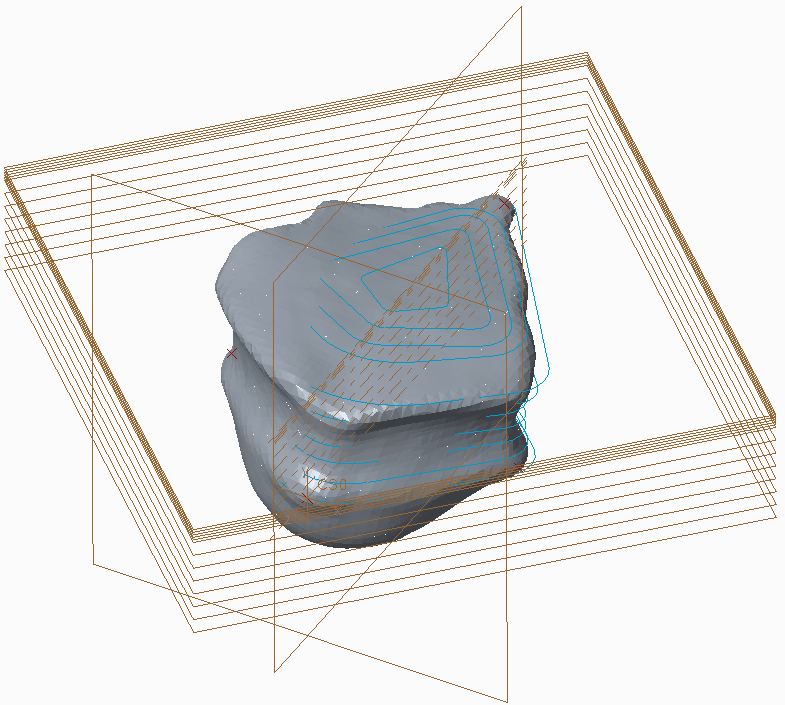
\includegraphics[width=7.8cm]{images/Scale_Replication_3.PNG}}\hfill
\vcenteredhbox{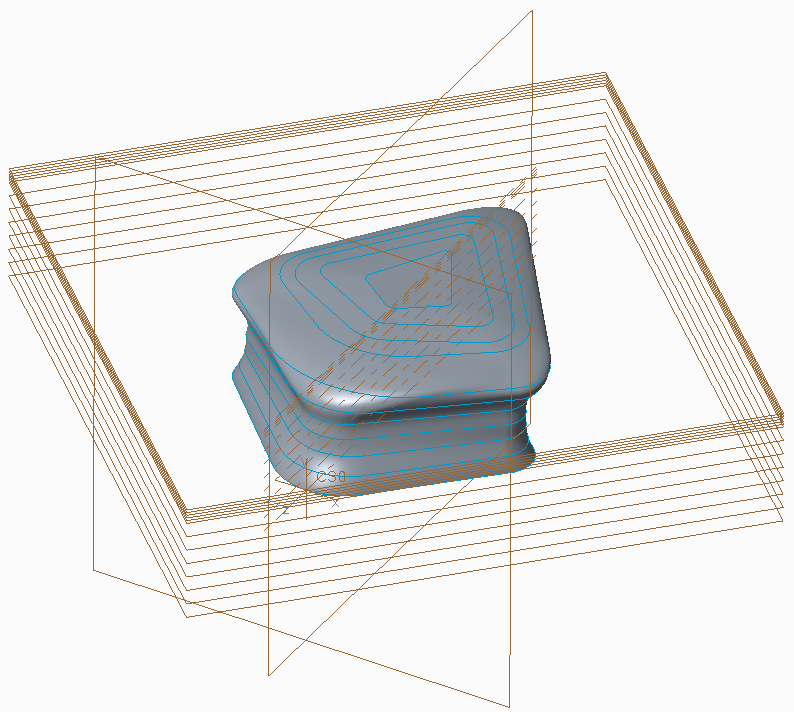
\includegraphics[width=7.8cm]{images/Scale_Replication_9.PNG}}
\caption{Comparison of sampled scale (left) and simplified scale (right) with overlaying primitive cross sections displayed.}
\label{figure:blendedScale}
\end{figure}

\begin{figure}[!b]
\centering
\vcenteredhbox{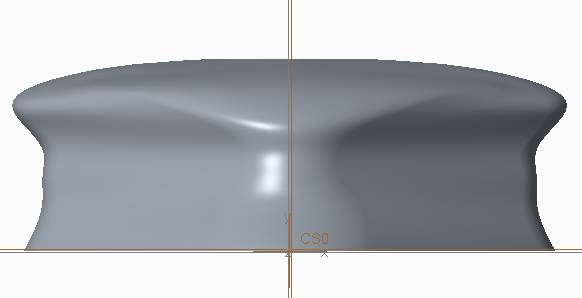
\includegraphics[width=7cm]{images/Scale_Replication_10.PNG}}\hfill
\vcenteredhbox{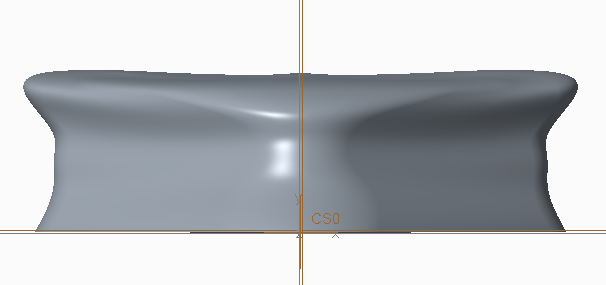
\includegraphics[width=7.5cm]{images/Scale_Replication_11.PNG}}
\caption{Comparison of blended scale (left) and warped scale (right).}
\label{figure:warping}
\end{figure}

\begin{figure}[!t]
\centering
\vcenteredhbox{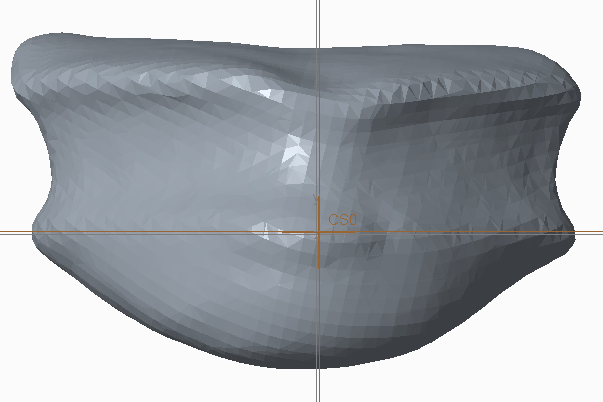
\includegraphics[width=7.5cm]{images/Scale_Replication_15.PNG}}\hfill
\vcenteredhbox{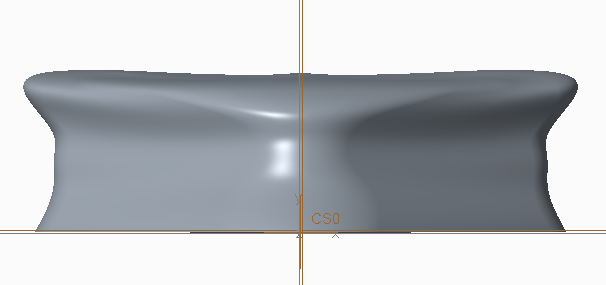
\includegraphics[width=7.5cm]{images/Scale_Replication_11.PNG}}
\\
\vspace{2cm}
\vcenteredhbox{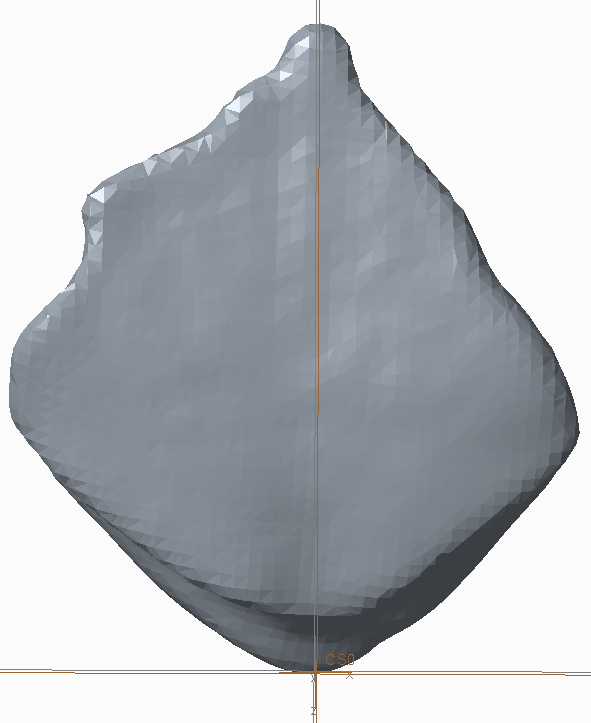
\includegraphics[width=7.5cm]{images/Scale_Replication_16.PNG}}\hfill
\vcenteredhbox{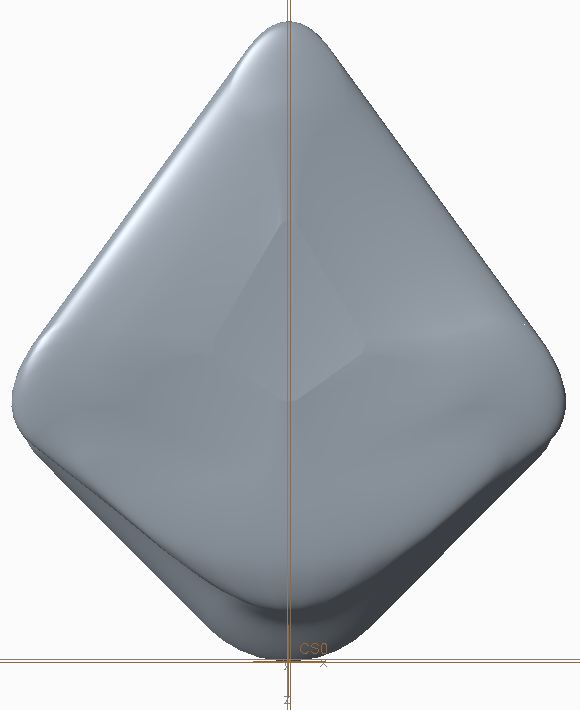
\includegraphics[width=7.5cm]{images/Scale_Replication_12.PNG}}
\\
\vspace{2.5cm}
\vcenteredhbox{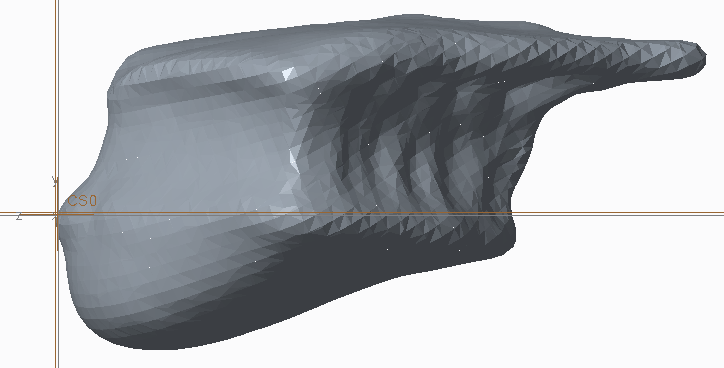
\includegraphics[width=7.5cm]{images/Scale_Replication_14.PNG}}\hfill
\vcenteredhbox{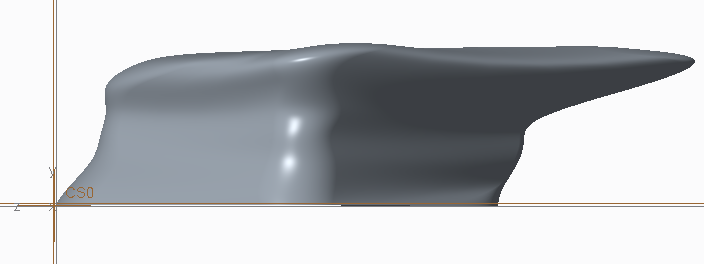
\includegraphics[width=7.5cm]{images/Scale_Replication_13.PNG}}
\caption{Comparison of sampled scale (left) and simplified scale (right).}
\label{figure:scaleComparison}
\end{figure}

\begin{figure}[!t]
\centering
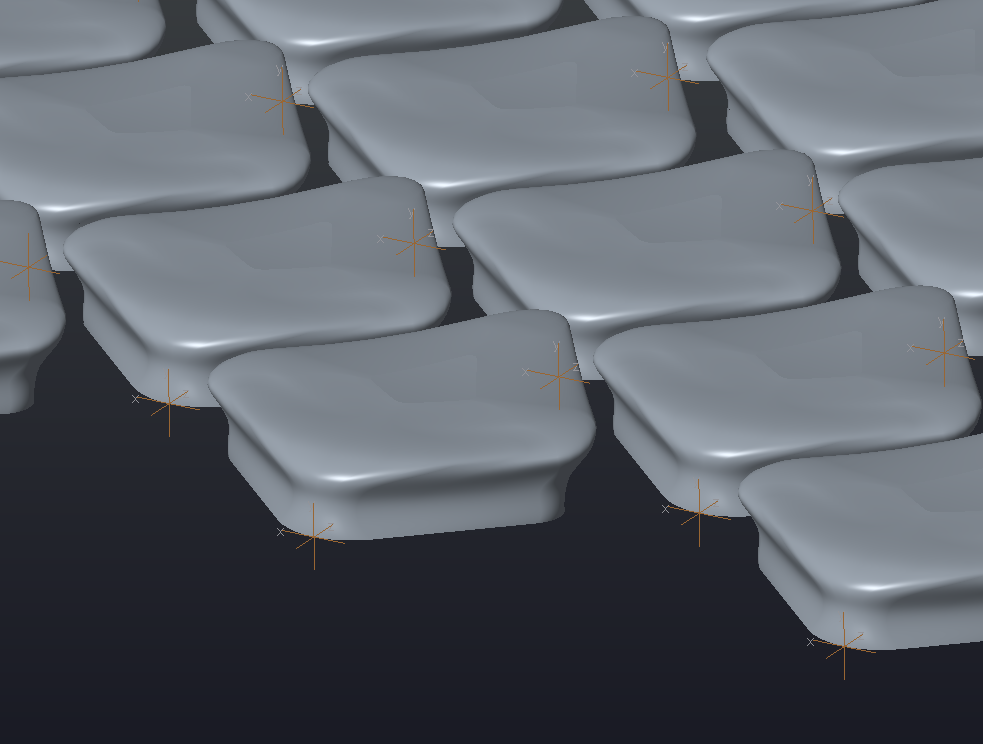
\includegraphics[width=7.5cm]{images/array_progress_report.PNG}
\caption{Array of staggered scales for 3D printing.}
\label{figure:staggeredArray}
\end{figure}




\newpage
\subsection{Preliminary Meshing Experiments}
\label{section:meshing}
The meshing process is a large factor in optimising a parametric CFD study: being able to generate a high quality mesh without user interaction would cut simulation time significantly. In addition to this, the periodicity must be exploited by the CFD solver, thus periodic boundaries must be treated by the meshing software. An example of the periodic domain is displayed in Figure \ref{figure:periodicDomain}, meshed using STAR-CCM+. The scale array can be reconstructed by copying and translating the domain in the $z$ direction and mirroring the domain in the $x$ direction. Several other meshing packages have been investigated since September and assessed via the following criteria:

\begin{figure}[!b]
\centering
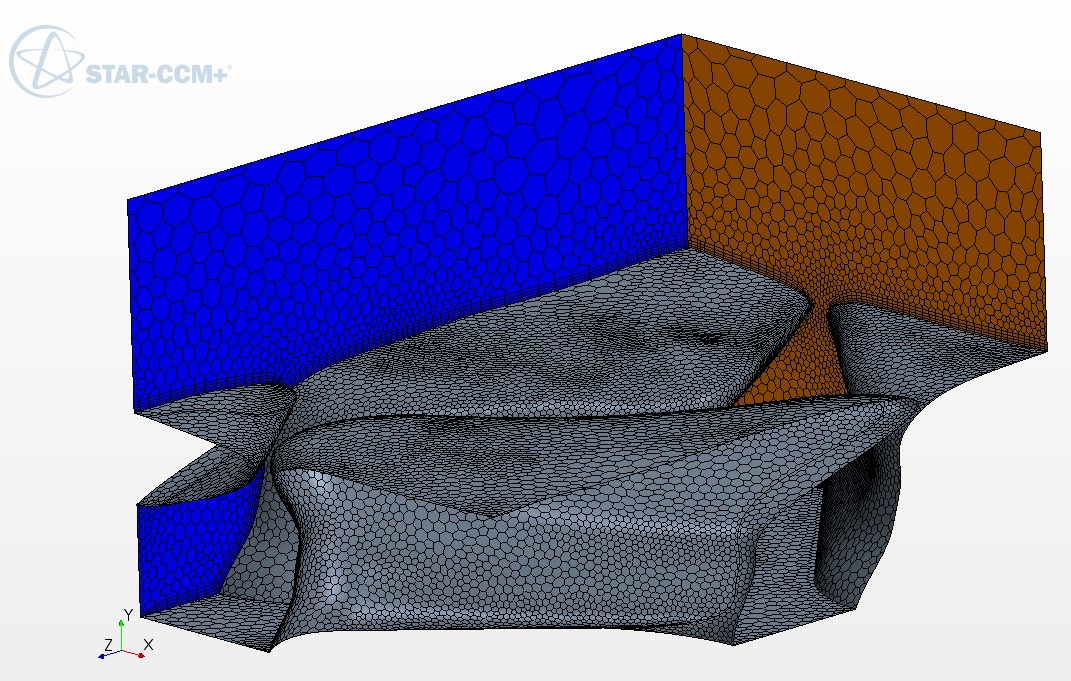
\includegraphics[width=12cm]{images/starccm_periodic_mesh.png}
\caption{Periodic mesh, created in STAR-CCM+, using the CAD scale documented in Section \ref{section:cad}. Periodicity exists between the $xz$ boundaries while symmetry planes are placed in the $yz$ planes.}
\label{figure:periodicDomain}
\end{figure}

\begin{itemize}
\itemsep0em
\item 
\textbf{Treatment of periodic boundaries}: Translational periodic boundaries can be applied by assuming the flow domain is infinitely long in the mean flow direction. Cell values are mapped between the two boundaries which requires their positions to be identical but translated downstream. When complex shapes, such as fish scales, intersect with these boundaries the meshing process becomes non-trivial. If the cell locations are identical then a `conformal' periodic boundary can be applied, otherwise `non-conformal' conditions are required. A non-conformal periodic boundary requires interpolation between faces, reducing the accuracy of the numerical scheme and introducing diffusive properties over the interface. 

\item 
\textbf{Cell types}: There are three common types of cells that are used for finite volume discretisation; hexahedral (6 faces), tetrahedral (4 faces), and polyhedral (arbitrary face count) \citep{durbin2007}. Hexahedral meshes are very common for simple geometric problems since it is straightforward to implement and maintain a high cell quality. However, fitting hexahedral cells to complex surfaces is non-trivial, making tetrahedral elements more suitable due to their flexibility, but with a compromise to numerical accuracy and convergence properties. In principle polyhedral cells can offer very smooth and high quality meshes, but they are generally more complex to create \citep{durbin2007}. Taking these into account, the desired meshing solver will contain polyhedral cells close to the fish scale surface, but blend into hexahedral cells, due to the simplicity of the rest of the channel domain. 

\item
\textbf{Scriptability}:
In order to reduce time, the meshing software used for the parameter study should be made scriptable to remove unnecessary user interaction. This would also allow small changes to be made to the CAD scale without requiring a new mesh case to be set up. This is less important for the LES model since only a single set of scales will be simulated.

\end{itemize}

Several software packages have been investigated, including both commercial and open source codes, which are summarised in Table \ref{table:meshSoftwareComparisons}. Advantages and disadvantages are present with each software, thus a compromise must be made when selecting a meshing package for both the LES case and the parametric study.

\begin{table}[!t]
\centering
\caption{Summary of tested meshing software in relation to the specified requirements of Section \ref{section:meshing}.}
\label{table:meshSoftwareComparisons}
\begin{tabular}{p{0.45\linewidth}p{0.45\linewidth}}
&\\
\textbf{ANSYS Fluent}	&	\\
\hline
\textbf{Pros}	&	\textbf{Cons}	\\
$\bullet$ High quality polyhedral cell mesh can be achieved,
&
$\bullet$ No blending between different cell types,
\\

$\bullet$ Mesher directly links to fluid solver,
&
$\bullet$ Conformal boundaries cannot be trivially set up.
\\

$\bullet$ Text based commands can be used and scripted, although this utility has not been investigated.
&
\\&\\	

\textbf{ANSYS ICEM CFD}	&	\\
\hline
\textbf{Pros}	&	\textbf{Cons}	\\
$\bullet$	High quality structured meshes can be achieved,
&
$\bullet$	Conformal boundaries cannot be trivially achieved,
\\
$\bullet$	Cell types can be blended (Hex. and Tet.),
&
$\bullet$	cannot create polyhedral cells.
\\
$\bullet$	Scriptable process.
&
\\&\\

\textbf{ANSYS Meshing}	&	\\
\hline
\textbf{Pros}	&	\textbf{Cons}	\\
$\bullet$ 	Scriptable through workbench,
&
$\bullet$	Little control over mesh quality,
\\
$\bullet$	can blend Hex. and Tet. cells.
&
$\bullet$	no polyhedral cells,
\\&\\

\textbf{STAR-CCM+}	&	\\
\hline
\textbf{Pros}	&	\textbf{Cons}	\\
$\bullet$ 	Primarily used for polyhedral meshing,
&
$\bullet$	Little control over quality and mesh refinement,
\\
$\bullet$	links to both inbuilt CAD for domain specification and CFD solver,
&
$\bullet$	No blending between different cell types.
\\
$\bullet$	Conformal boundaries are trivial to set up.
&
\\&\\

\textbf{SnappyHexMesh}	&	\\
\hline
\textbf{Pros}	&	\textbf{Cons}	\\
$\bullet$	Intuitive scriptability with effective link to OpenFOAM solver,
&
$\bullet$ Requires a lot of parameter tuning to generate an initial script,
\\
$\bullet$	full control over cell quality and refinement regions,
&
$\bullet$ requires a high quality .stl CAD file to generate a good quality mesh.
\\
$\bullet$	Primarily hexahedral cells but blends into polyhedral cells on complex surfaces.
&
$\bullet$	Complex features on periodic interfaces are non-conformal, but this can be blended into a conformal boundary further from this surface,

\end{tabular}
\end{table}

Both STAR-CCM+ and SnappyHexMesh have significant advantages over the other tested packages; STAR-CCM+ allows the generation of a smooth polyhedral mesh with conformal boundaries but requires more user interaction to ensure the mesh quality is appropriate. SnappyHexMesh is naturally scriptable and enforces specified quality criteria. However, a mix of conformal and non-conformal boundary conditions are required for the algorithm to work properly. For this reason, the high resolution LES model will be implemented using a polyhedral mesh, specified in STAR-CCM+. The parameter study will be carried out using SnappyHexMesh. Both sets of simulations will be carried out using the OpenFOAM fluid solver.

In terms of mesh generation, work over the following 6 months will consist of performing LES on a polyhedral mesh, in order to determine appropriate solver and discretisation settings to achieve comparable results to those presented in Section \ref{section:les}. In addition to this, appropriate mesh parameters will be determined for the SnappyHexMesh case and RANS simulations will be carried out on this domain to assess mesh independence and the influence of RANS model choice on the solution. This information will be used to create an appropriate sizing for the LES mesh.

\newpage
\subsection{Application of Reynolds-Averaged Navier-Stokes to a periodic shark scale domain}
\label{section:rans}
Dependency analysis of RANS methods on a periodic shark scale domain.
Dependencies include MI, DI, model I, Numerics I, Tol I ...
The results will form the basis for the mesh resolution for the LES and the RANS studies. Before carrying out further RANS the results will be validated against a LES. 

\subsubsection{Problem definition}
As discussed? The Reynolds equations are given by

\begin{equation}
\frac{\overline{D} \langle U_i \rangle }{ \overline{D} t}
=
-\pdev{\langle P \rangle}{x_i}
+
\nu
	\left(
	\pdev{\langle U_j \rangle}{x_i}
	+
	\pdev{\langle U_i \rangle}{x_j} 
	\right)
+
\pdev{\langle u_i u_j\rangle}{x_i}.
\end{equation}
and the continuity equation by

\begin{equation}
\pdev{\langle U_i\rangle}{x_i}=0,
\end{equation}
where $\langle \phi \rangle$ represents the ensemble average of $\phi$. The present work adopts the turbulent viscosity hypothesis whereby the Reynolds stresses are estimated using

\begin{equation}
\left< u_i u_j \right> = \frac{2}{3}k \delta_{ij} - \nu_T \left( 
	\pdev{\left< U_i \right>}{x_j} + \pdev{\left< U_j \right>}{x_i}	\right).
\end{equation}

In order to model $\nu_T$ the model of (REF) is adopted, whereby transport equations for $k$, the turbulent kinetic energy, and $\omega$, the ...? are solved. 


These equations are similar in appearance as the Navier-Stokes equations \eqref{equation:fundamentalEquations:momentum} but require information about the Reynolds stresses, $\langle u_i u_j \rangle$. This forms the basis of the RANS ideology, whereby \eqref{equation:fundamentalEquations:meanContinuity} and \eqref{equation:fundamentalEquations:ReynoldsEquations} are solved for $\langle U_i \rangle$ and $\langle P \rangle$ by modelling the Reynolds stresses. There have been many proposed models to close this system of equations with varying accuracy and expense. A widely adopted approach to modelling these stresses is the turbulent-viscosity hypothesis which assumes
\begin{equation}
\left< u_i u_j \right> = \frac{2}{3}k \delta_{ij} - \nu_T \left( 
	\pdev{\left< U_i \right>}{x_j} + \pdev{\left< U_j \right>}{x_i}	\right),
\end{equation}
where $\nu_T(\boldsymbol{x},t)$ is the turbulent viscosity, analogous to the molecular viscosity. Algebraic relationships for $\nu_T$ have been suggested, such that $\nu_T=l_m^2 \left| (\partial \left<U\right> / \partial y   \right|$, but these are reliant on the specification of the mixing length $l_m$. 

\begin{equation}
\nu_T = c k^{1/2} l_m = C_\mu k^2/\epsilon,
\end{equation}


\begin{equation}
\pdev{k}{t} + \left< U_i \right> \cdot \nabla k = -\nabla \cdot T_i' + \mathcal{P} - \epsilon 
\end{equation}

\begin{equation}
T_i' = \frac{1}{2} \left< u_i u_j u_j \right> + \left< u_i P' \right> - 2 \nu \left< u_j s_{ij} \right>.
\end{equation}
where $P'$ is the fluctuation component of the kinematic pressure. Further assumptions: the flux, $T_i'$ is modelled using gradient diffusion, i.e 
\begin{equation}
T_i' = -\frac{\nu_T}{\sigma_{k}} \nabla k,
\end{equation}
where the turbulent Prandtl number is generally taken as $\sigma_k=1$. This physically asserts that due to velocity and pressure fluctuations there is a flux of k down the gradient of k \citep{pope2001}.

The equation for omega is entirely empirical:
\begin{equation}
\pdev{\omega}{t}  + \left< U_i \right> \cdot \nabla \omega = \nabla \cdot \left( \frac{\nu_T}{\sigma_{\omega}} \nabla \omega \right) + C_{\omega 1} \frac{\mathcal{P} \omega}{k} - C_{\omega 2} \omega^2
\end{equation}
By taking $\omega \equiv \epsilon /k$ and substituting into $\epsilon$ equation we get
\begin{equation}
\pdev{\omega}{t}  + \left< U_i \right> \cdot \nabla \omega = \nabla \cdot \left( \frac{\nu_T}{\sigma_{\epsilon}} \nabla \omega \right) + (C_{\varepsilon 1}-1) \frac{\mathcal{P} \omega}{k} - (C_{\varepsilon 2}-1) \omega^2 + \frac{2 \nu_T}{\sigma_\epsilon k}\nabla \omega \cdot \nabla k
\end{equation}


-present k and epsilon equations
-indicate what each term is - including the weighting factor
-Then introduce the FV method and how equations are discretised over our domain - BC. 


\newpage

\subsubsection{Results and discussion}

%PROFILES: Ux
\begin{figure}[!h]
\centering
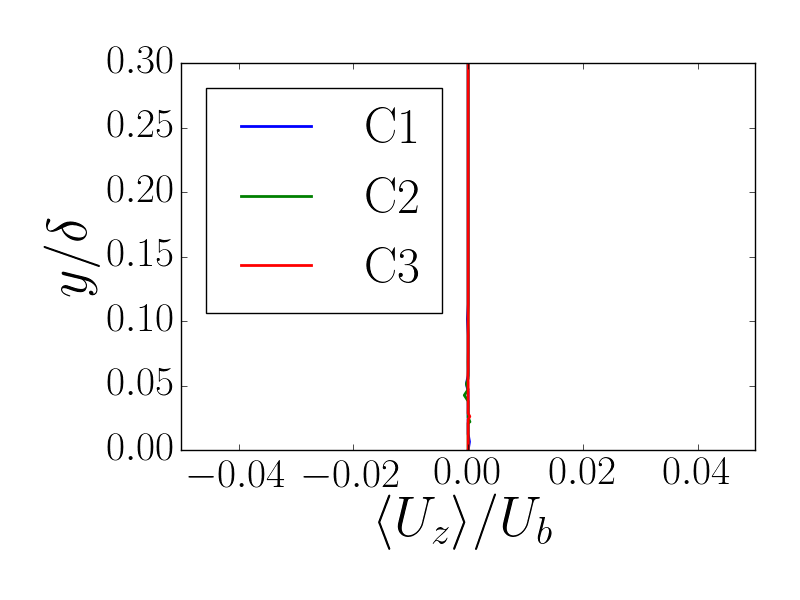
\includegraphics[width=7.5cm]{images/CFD_meshIndependence/X1_Ux.png}\hfill 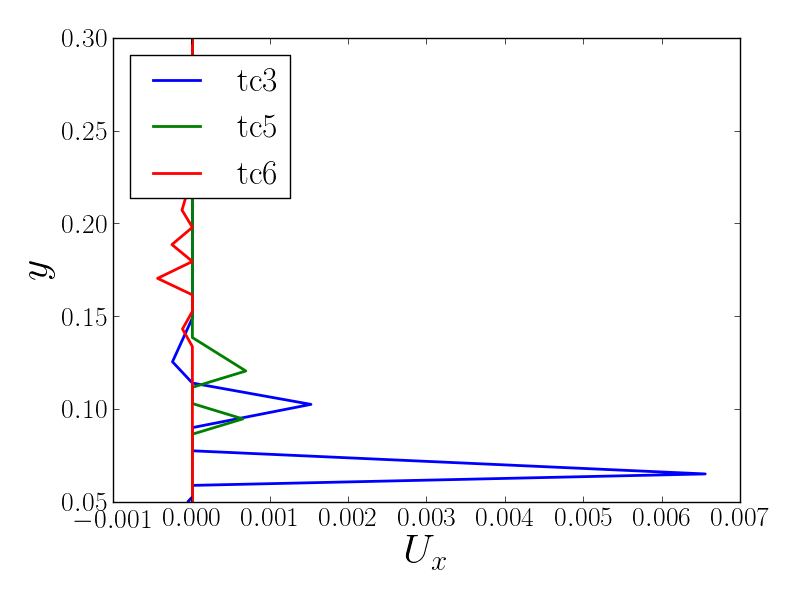
\includegraphics[width=7.5cm]{images/CFD_meshIndependence/X2_Ux.png}\\
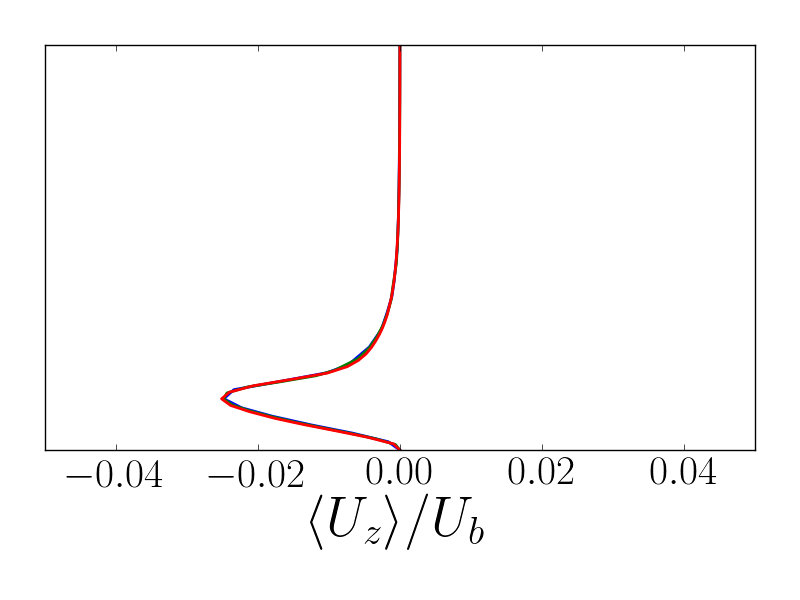
\includegraphics[width=7.5cm]{images/CFD_meshIndependence/X3_Ux.png}
\end{figure}

%PROFILES: Uy
\begin{figure}
\centering
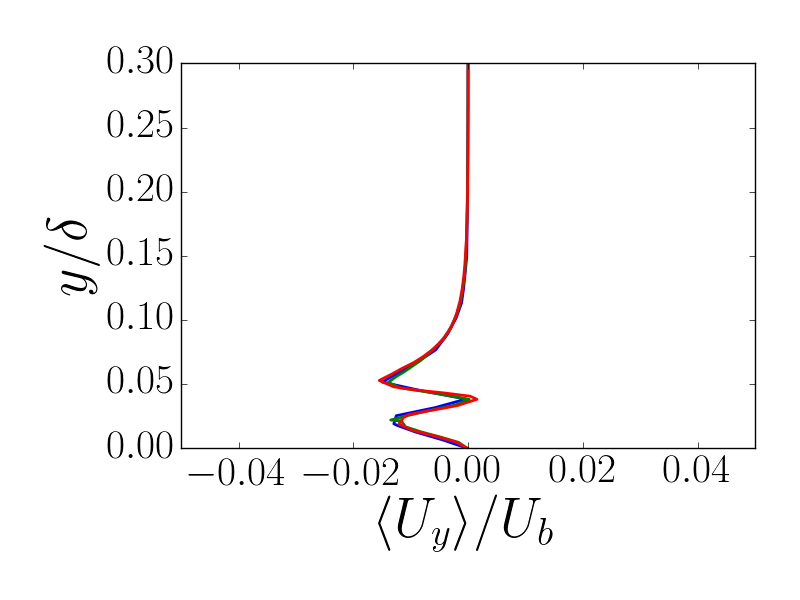
\includegraphics[width=7.5cm]{images/CFD_meshIndependence/X1_Uy.png}\hfill 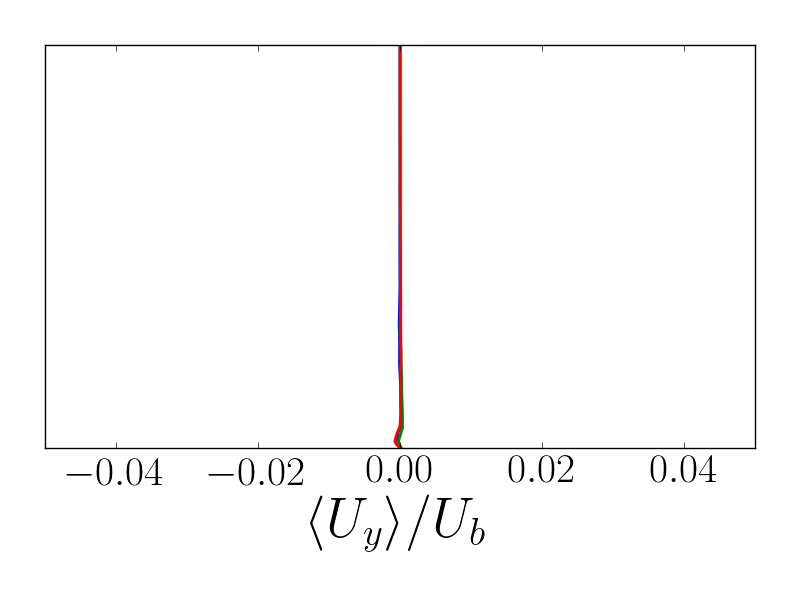
\includegraphics[width=7.5cm]{images/CFD_meshIndependence/X2_Uy.png}\\
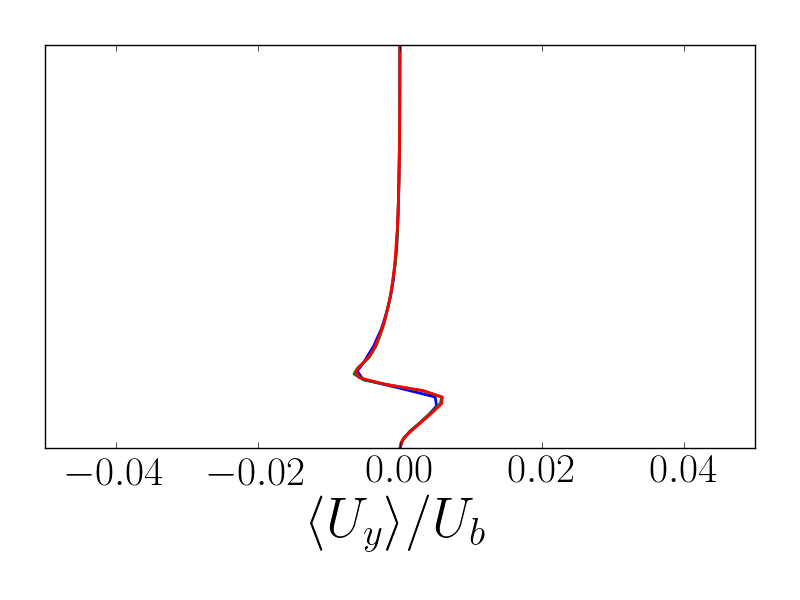
\includegraphics[width=7.5cm]{images/CFD_meshIndependence/X3_Uy.png}
\end{figure}

%PROFILES: Uz
\begin{figure}
\centering
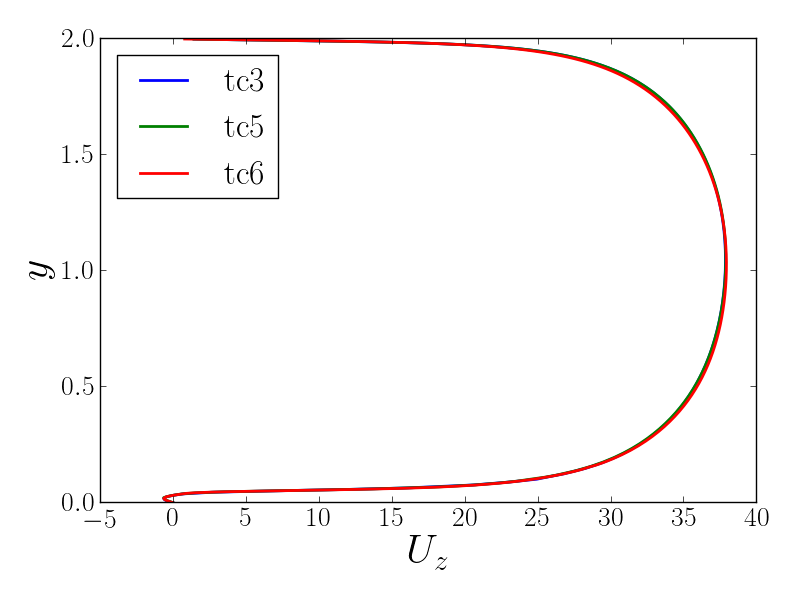
\includegraphics[width=7.5cm]{images/CFD_meshIndependence/X1_Uz.png}\hfill 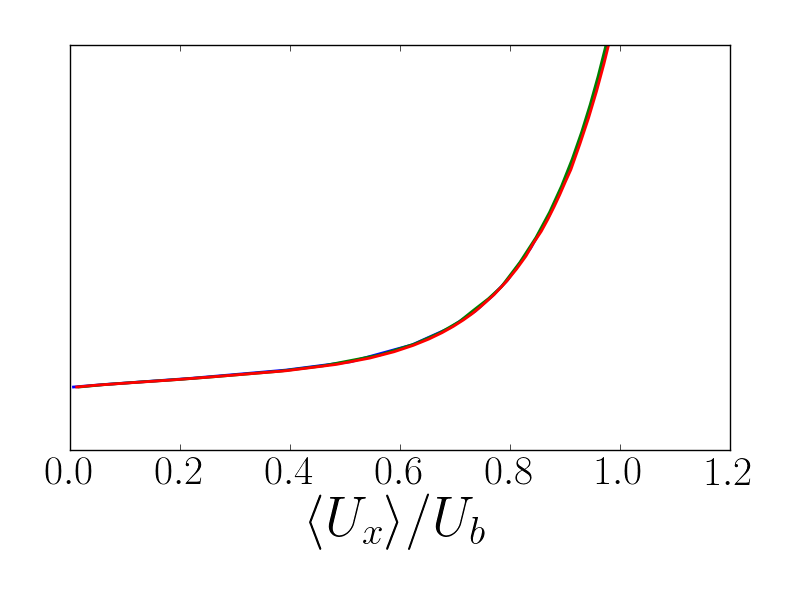
\includegraphics[width=7.5cm]{images/CFD_meshIndependence/X2_Uz.png}\\
\includegraphics[width=7.5cm]{images/CFD_meshIndependence/X3_Uz.png}
\end{figure}

%PROFILES: magGradU
\begin{figure}
\centering
\includegraphics[width=7.5cm]{images/CFD_meshIndependence/X1_gradU.png}\hfill \includegraphics[width=7.5cm]{images/CFD_meshIndependence/X2_gradU.png}\\
\includegraphics[width=7.5cm]{images/CFD_meshIndependence/X3_gradU.png}
\end{figure}

%PROFILES: p
\begin{figure}
\centering
\includegraphics[width=7.5cm]{images/CFD_meshIndependence/X1_p.png}\hfill \includegraphics[width=7.5cm]{images/CFD_meshIndependence/X2_p.png}\\
\includegraphics[width=7.5cm]{images/CFD_meshIndependence/X3_p.png}
\end{figure}

%PROFILES: k
\begin{figure}
\centering
\includegraphics[width=7.5cm]{images/CFD_meshIndependence/X1_k.png}\hfill \includegraphics[width=7.5cm]{images/CFD_meshIndependence/X2_k.png}\\
\includegraphics[width=7.5cm]{images/CFD_meshIndependence/X3_k.png}
\end{figure}

%PROFILES: omega
\begin{figure}
\centering
\includegraphics[width=7.5cm]{images/CFD_meshIndependence/X1_omega.png}\hfill \includegraphics[width=7.5cm]{images/CFD_meshIndependence/X2_omega.png}\\
\includegraphics[width=7.5cm]{images/CFD_meshIndependence/X3_omega.png}
\end{figure}


Contour plots:
For a scalar, $\phi$, we assess independence by interpolating the solution over the scale surface onto the finest STL scale surface. This ensures that cells coincide and solutions can be directly compared. The reference scalar $\phi_{REF}$ is the solution of the finest mesh. It is scaled such that its minimum value is 0 and maximum is 1:
\begin{equation}
\overline{\phi}_{\text{REF}} = \frac{\phi_{\text{REF}}-\text{min}(\phi_{\text{REF}})}{\text{max}(\phi_{\text{REF}})-\text{min}(\phi_{\text{REF}})}.
\end{equation}
Similarly, $\phi$, the coarse mesh solution, is translated to a minimum value of 0 and then scaled by the same amount as $\phi_{\text{REF}}$:
\begin{equation}
\overline{\phi} = \frac{\phi-\text{min}(\phi)}{\text{max}(\phi_{\text{REF}})-\text{min}(\phi_{\text{REF}})}.
\end{equation}
The error is defined as the root-mean-square of the difference between $\phi$ and $\phi_{\text{REF}}$:
\begin{equation}
\text{error}(\phi)\sqrt{(\overline{\phi}_{\text{REF}} - \overline{\phi})^2}
\end{equation}


%contour plots: pressure
\begin{figure}
\centering
\includegraphics[height=3.1cm]{images/CFD_meshIndependence/tc3_p.png}\hfill \includegraphics[height=3.1cm]{images/CFD_meshIndependence/tc5_p_bar.png}
\end{figure}

%contour plots: gradU
\begin{figure}
\centering
\includegraphics[height=3.1cm]{images/CFD_meshIndependence/tc3_gradU.png}\hfill \includegraphics[height=3.1cm]{images/CFD_meshIndependence/tc5_gradU_bar.png}\\
\end{figure}


\newpage
Introduction: - what are we doing, why, how ..
dependency studies
-MI, DI, models, tolerances, disc. schemes etc. 
-Eventually validate against LES 
-Then we can start varying parameters to see effects on the flow field
Methodology: - meshing parameters and models used
- show domain and BCs,
-numerical methods,
Results: - MI results for contour plots over surface, profile plots in wall-normal direction.


\newpage
\subsection{Large eddy simulation of a channel flow}
\label{section:les}
In order to exploit periodicity, an infinitely long and wide channel flow with scales on one wall will be simulated. Large-eddy simulation will be adopted in order to model the flow at a feasibly high resolution for a bulk Reynolds number greater than $Re_b = 20\ 000$. The precise Reynolds number will be determined later this year when designing the LDA experiments. Before implementing the LES on a channel flow with scales, the code is validated with smooth walls. This is carried out at a low Reynolds number of $Re_\tau = 180$ to make use of the extensive DNS database of \cite{vreman2014}. By validating at this Reynolds number we can determine suitable model and solver parameters without requiring extensive computing costs. Over the following year the model will be extended to a high Reynolds number to provide a base case for both comparisons against fish scale surfaces, and an estimation of the number of cells required.

\subsubsection{Mathematical Model}
\label{section:mathematicalModel}
Large eddy simulation is a technique used to study turbulence whereby the large turbulent structures are resolved and the small structures are modelled as a stress term. This is achieved by decomposing the velocity field into a filtered and residual term so that $\vecti{U} = \overline{\vecti{U}} + \vecti{u}'$. The filtered momentum (\ref{equation:momentum}) and continuity (\ref{equation:continuity}) equations \citep{pope2001} are defined as
\begin{equation}
\label{equation:momentum}
\pdev{\vecti{\overline{U}}}{t} + \pdev{\vecti{\overline{U}} \vectj{\overline{U}}}{\vectj{x}} - \pdev{}{\vectj{x}}(\matij{\overline{\sigma}} + \matij{\tau}) = - \pdev{\overline{P}}{\vecti{x}},
\end{equation}
and
\begin{equation}
\label{equation:continuity}
\pdev{\vecti{\overline{U}}}{\vecti{x}} = 0,
\end{equation}
where $\matij{\overline{\sigma}} = 2\nu \matij{\overline{S}}$ represents the resolved viscous stress tensor, $\overline{P} = \overline{p}/\rho$ is the resolved kinematic pressure, and $\matij{\overline{S}} = \frac{1}{2}\left( \pdev{\vecti{\overline{U}}}{\vectj{x}} + \pdev{\vectj{\overline{U}}}{\vecti{x}} \right)$ is the filtered rate of strain tensor. $\tau_{ij} = \vecti{\overline{U}} \vectj{\overline{U}} - \overline{\vecti{U} \vectj{U}}$ represents the effect of the unfiltered velocity field on the filtered field. This may be approximated using the model of \cite{smagorinsky1963}:
\begin{equation}
\label{equation:tau}
\matij{\tau}-\frac{1}{3}\matij{\delta}\tau_{kk} = 2\nu_{t} \matij{\overline{S}},
\end{equation}
where $\nu_t$ is the sub-grid scale viscosity. \cite{smagorinsky1963} defines this sub-grid scale viscosity as
\begin{equation}
\label{equation:smagorinsky}
\nu_t = (C_s \Delta)^2 |\overline{S}|,
\end{equation}
where $C_s$ is the Smagorinsky constant and $\Delta$ is the filter width, based on the local grid size. The magnitude of the filtered rate of strain tensor is defined as $|\overline{S}|= (2 \matij{\overline{S}} \matij{\overline{S}})^{1/2}$. The Smagorinsky model assumes a constant value of $C_s = 0.17$ \citep{smagorinsky1963}. However, the assumption that $C_s$ does not vary in space or time is a strong limitation to the model, as will be further discussed in section \ref{section:lesResults}. An alternative method, first suggested by \cite{germano1991}, estimates the coefficient by filtering \eqref{equation:momentum} and \eqref{equation:continuity} a second time. By applying this filter we can define an addition stress term, equivalent to (\ref{equation:tau}) just on a coarser grid of filter width $\widetilde{\Delta} = 2\Delta$: $\matij{T}-\frac{1}{3}\matij{\delta}T_{kk} =\vecti{\widetilde{\overline{U}}}\vectj{\widetilde{\overline{U}}}-\widetilde{\overline{\vecti{U}\vectj{U}}}$. By adopting the Germano identity \citep{germano1991}, we relate the scales of motion between the two filter widths:
\begin{equation}
\label{equation:germano}
\matij{L} = \matij{T}^r - \matij{\widetilde{\tau}}^r = \vecti{\widetilde{\overline{U}}}\vectj{\widetilde{\overline{U}}} - \widetilde{\vecti{\overline{U}}\vectj{\overline{U}}}.
\end{equation}
Unlike the equations for $\tau_{ij}$ and $T_{ij}$, equation \ref{equation:germano} can be solved from the filtered velocity field.  Assuming $\matij{T}$ takes the same form as $\matij{\tau}$, $L_{ij}$ can be solved to find $C_s$:
\begin{equation}
L_{ij} = 2\Delta^2 \left[	\widetilde{C_s^2 |\overline{S} | \matij{\overline{S}}} - 4 C_s^2 |\widetilde{\overline{S}}| \matij{\widetilde{\overline{S}}}		 \right].
\end{equation}
This represents 5 equations with 1 unknown, the error of which is given by
\begin{equation}
\label{equation:CsError}
e_{ij} = 	L_{ij} - M_{ij}C_s^2			,
\end{equation}
where $$M_{ij} =  2\Delta^2 \left[	\widetilde{|\overline{S} | \matij{\overline{S}}} - 4 |\widetilde{\overline{S}}| \matij{\widetilde{\overline{S}}} \right].$$
It is assumed that the constant $C_s$ does not vary spatially between the scales $\Delta$ and $2\Delta$, allowing it to be taken out of the filter term.

Typically the error is minimised by differentiating equation (\ref{equation:CsError}) with respect to $C_s^2$. However, this method requires both spatial averaging, in homogeneous directions, and clipping, in order to ensure $C_s$ remains positive (energy dissipating). An alternative to this restrictive dynamic model is to average along particle paths using the model of \cite{meneveau1996}. In a Lagrangian frame of reference, the trajectory of a fluid particle for earlier times $t'<t$ is given by
\begin{equation}
\label{equation:particlePath}
\vect{z}(t') = \vect{x} - \int_{t'}^t \overline{\vect{u}}(\vect{z}(t''),t'')dt''.
\end{equation}
In terms of the Lagrangian description the error to be minimised, (\ref{equation:CsError}), is
\begin{equation}
\label{equation:lagrangianCsError}
e_{ij}(\vect{z},t') = 	L_{ij}(\vect{z},t') - M_{ij}(\vect{z},t')C_s^2(\vect{x},t'),
\end{equation}
where it is assumed that $C_s$ can be removed from the filter by assuming it does not vary strongly over the scale of the test filter, an assumption that is investigated and justified by \cite{meneveau1996}. In order to minimise this error we define the total error as the pathline accumulation of the local error squared, 
\begin{equation}
\label{equation:ErrorSquared}
E = \int_{-\infty}^t e_{ij}(\textbf{z}(t'),t')e_{ij}(\textbf{z}(t'),t') W(t-t') dt',
\end{equation}
where $W(t-t')$ is a weighting function, introduced in order to control the contributions from times closer to $t$. Differentiating with respect to $C_s^2$, and making use of (\ref{equation:lagrangianCsError}), we obtain
\begin{equation}
\label{equation:CsFlmFmm}
C_s^2(\vect{x},t) = \frac{f_{LM}}{f_{MM}},
\end{equation}
where
\begin{equation}
\label{equation:flm}
f_{LM} = \int_{-\infty}^t L_{ij}M_{ij}(\vect{z}(t'),t') W(t-t') dt',
\end{equation}
and
\begin{equation}
\label{equation:fmm}
f_{MM} = \int_{-\infty}^t M_{ij}M_{ij}(\vect{z}(t'),t') W(t-t') dt'.
\end{equation}
A convenient choice of the weighting function is $W(t-t')=T^{-1} e^{-(t-t')/T}$ \citep{meneveau1996}. This results in two transport equations for $f_{LM}$ and $f_{MM}$ rather than backward integrals in time:
\begin{equation}
\label{equation:flmTransport}
\frac{D f_{LM}}{Dt} = \frac{1}{T}(L_{ij}M_{ij} - f_{LM}),
\end{equation}
\begin{equation}
\label{equation:fmmTransport}
\frac{D f_{MM}}{Dt} = \frac{1}{T}(M_{ij}M_{ij} - f_{MM}).
\end{equation}
$T$ represents a timescale that controls the memory length. There are some natural choices for this parameter, highlighted by \cite{meneveau1996}, whereby the timescale can be controlled by the values of $f_{LM}$ and $f_{MM}$. By taking $T=\theta \Delta (f_{LM} f_{MM})^{-1/8}$, where $\theta$ is a constant of order unity, the memory time will be reduced in both regions of high straining (high $f_{MM}$) and large nonlinear energy transfer (high $f_{LM}$). Typically $\theta=1.5$ for most cases, although there is some solution dependence on this value. This dependency will be investigated in future work. 

With these parameters now defined, the transport equations (\ref{equation:flmTransport}) and (\ref{equation:fmmTransport}) can be solved and used to determine $C_s$. The turbulent stress tensor equation, (\ref{equation:tau}), can now be solved, closing our set of equations.

\subsubsection{Numerical Implementation}
The equations are solved using OpenFOAM, a finite volume platform. The equations are discretised over a channel of dimensions $4.2\delta \times 2\delta \times 12.6\delta$ where $\delta$ is the channel half height. Similar dimensions are used by several authors such as \cite{moser1999}, and \cite{vreman2014} for a Reynolds number of $Re_\tau = 180$, although the influence of domain size on the turbulent statistics is still poorly understood \citep{vreman2014}. Three simulations are presented in this report, one which which solves equations for only half the channel height and applies symmetry boundary conditions at the central plane, $y=\delta$. If validated, this model could reduce the number of required cells. The half channel simulation adopts a constant value of $C_s = 0.17$, validated against a full channel simulation using the same model. The final simulation adopts the dynamic Lagrangian model discussed in Section \ref{section:mathematicalModel}.

The mesh statistics are presented in Table \ref{table:meshStatistics}. The total number of cells is $\sim 4M$, much fewer than an equivalent finite difference DNS of \cite{vreman2014} who used $\sim 33M$ grid points. A Cosine distribution is adopted in the wall-normal direction in order to capture the large gradients close to the wall. The y-normal boundary conditions can be observed from Table \ref{table:boundaryConditions}. The boundary conditions for $f_{LM}$ and $f_{MM}$ are defined by \cite{meneveau1996}. Periodic boundary conditions are applied in both streamwise and spanwise direction with a forcing term added to the momentum equation (\ref{equation:momentum}) in order to maintain a constant bulk Reynolds number in the $z$ direction. The forcing term is derived by decomposing the pressure gradient into an average and fluctuating component; the average pressure gradient is adjusted each timestep in order to ensure a fixed mean velocity through the periodic faces, $ \overline{\vect{U}}_{ave} $. A description of this technique is presented by \cite{murthy1997}.

\begin{table}[!b]
\centering
\caption{Mesh statistics for the three LES cases. The half channel case takes $N_y = 64$}
\label{table:meshStatistics}
\begin{tabular}{|l|l|l|l|l|l|l|}
\hline
$N_x$  & $N_y$  & $N_z$  & $\Delta x^+$ & $\Delta z^+$ & $\Delta y^+_{min}$ & $\Delta y^+_{max}$ \\ \hline
$160$ & $128$ & $192$ & $4.7$     & $11.8$    & $0.18$           & $4.5          $ \\ \hline
\end{tabular}
\end{table}

A convenient choice for the parameters $\nu$ and $ \overline{\vect{U}}_{ave} $ will fix the bulk Reynolds number to $Re_b = 2800$, corresponding to a shear Reynolds number of $Re_\tau \approx 180$. The choice of fixing the bulk flow Reynolds number is more natural when considering the validation of further results against experiments later this year. For a channel flow, $Re_\tau$ can be determined from the pressure gradient over the periodic boundary by applying a force balance over the domain:
$$	Re_\tau = u_\tau \delta / \nu, \hspace{1cm} u_\tau = \sqrt{\tau_w / \rho},	\hspace{1cm}	\tau_w / \rho = \delta \pdev{P}{z}\bigg\vert_{ave}. 	$$
A convenient choice of parameters are $\delta = 1$ and $\nu = 1/180$ resulting in an average shear velocity of $u_\tau \approx 1$ and $Re_\tau \approx 180$. The initial state makes use of a perturbation utility in OpenFOAM which adds instabilities to a flow profile of mean velocity $ \overline{\vect{U}}_{ave} $. These instabilities grow between timesteps until a statistically steady and turbulent state is present. 

\begin{table}[!t]
\centering
\caption{Boundary conditions for the three LES cases.}
\label{table:boundaryConditions}
\begin{tabular}{ll|l|l|}
\cline{3-4}
                                                                                                             &           & $y=0$, $y=2\delta$ (full channel) & $y=\delta$ (half channel) \\ \cline{2-4} 
\multicolumn{1}{l|}{}                                                                                        & Variable  & Condition                         & Condition                 \\ \hline
\multicolumn{1}{|l|}{Half channel}                                                                           & $U$       & Dirichlet                         & Neumann                   \\
\multicolumn{1}{|l|}{}                                                                                       & $P$       & Neumann                           & Neumann                   \\
\multicolumn{1}{|l|}{}                                                                                       & $\nu_{t}$ & Neumann                           & Neumann                   \\ \hline
\multicolumn{1}{|l|}{Full channel}                                                                           & $U$       & Dirichlet                         & -                         \\
\multicolumn{1}{|l|}{}                                                                                       & $P$       & Neumann                           & -                         \\
\multicolumn{1}{|l|}{(Smagorinsky Model)}                                                                    & $\nu_{t}$ & Neumann                           & -                         \\
\multicolumn{1}{|l|}{\multirow{2}{*}{\begin{tabular}[c]{@{}l@{}}(Dynamic\\  Lagrangian Model)\end{tabular}}} & $f_{LM}$  & Dirichlet                         & -                         \\
\multicolumn{1}{|l|}{}                                                                                       & $f_{MM}$  & Neumann                           & -                         \\ \hline
\end{tabular}
\end{table}

The momentum (\ref{equation:momentum}), continuity (\ref{equation:continuity}), and the two Lagrangian transport equations (\ref{equation:flmTransport}) and (\ref{equation:fmmTransport}) are discretised using second order schemes in both space and time. Backward Euler is adopted for discretisation in time and Gaussian integration in space. Linear interpolation is adopted in order to interpolate values from cell centres to cell faces. The PISO algorithm (Pressure-Implicit with Splitting of Operators) of \cite{issa1986} is adopted, whereby a pressure equation is derived from the momentum (\ref{equation:momentum}) and continuity equations (\ref{equation:continuity}). The PISO scheme operates using a two-step process: A predictor step and a corrector step. The semi-discrete form of (\ref{equation:momentum}) can be written as
\begin{equation}
\label{equation:piso1}
\vect{C} \vect{u}^* =  \vect{A}\vect{u}^* + \vect{H'}\vect{u}^* =\vect{r} - \nabla \vect{P}^n,
\end{equation} 
where $\vect{C}$ represents the implicit coefficient array, $\vect{u}^*$ is the predicted velocity, $\vect{r}$ is the explicit source terms and $\vect{P}^n$ represents the kinematic pressure at the previous time step. The matrix $\vect{C}$ can be split into diagonal and off diagonal components, $\vect{C} = \vect{A} + \vect{H'}$, and the linear equation (\ref{equation:piso1}) can be solved for $\vect{u}^*$. A Gauss-Seidel solver is adopted to solve this system, completing the predictor step. (\ref{equation:piso1}) can be manipulated in order to derive an equation to correct both the velocity and pressure from the predicted velocity:
\begin{equation}
\label{equation:piso2}
\vect{A}\vect{u}^{**} + \vect{H'}\vect{u}^* =\vect{r} - \nabla \vect{P}^*,
\end{equation}
\begin{equation}
\label{equation:piso3}
\vect{u}^{**}  = \vect{A}^{-1}\vect{H} - \vect{A}^{-1}\nabla \vect{P}^*,
\end{equation}
where $\vect{H} = \vect{r} - \vect{H'}\vect{u}^*$. The inversion of $\vect{A}$ is trivial since it is symmetrical. By recognising that $\nabla \vect{u}^{**} = 0$, a Poisson equation for the corrected pressure can be derived:
\begin{equation}
\label{equation:piso4}
\nabla^2 ( \vect{A}^{-1} \vect{P}^* ) = \nabla \cdot (\vect{A}^{-1} \vect{H}).
\end{equation}
This Laplacian equation is solved using a Geometric-algebraic multi-grid solver in order to update the pressure. The corrected velocity equation (\ref{equation:piso3}) is then solved to update the velocity. In order to ensure second order accuracy, (\ref{equation:piso4}) and (\ref{equation:piso3}) and solved twice, as recommended by \cite{issa1986}. Equations (\ref{equation:flmTransport}) and (\ref{equation:fmmTransport}) are discretised using the same method as the momentum equation and solved using a Gauss-Seidel solver. All equations are iteratively solved until a tolerance of $10^{-8}$ is met. An adaptive time-stepping scheme is adopted in order to ensure the Courant number does not exceed $0.5$. Statistical averaging is carried out between the time intervals $t=10 \delta / u_\tau$ and $t = 40 \delta / u_\tau$. This interval is much smaller than those adopted by \cite{kim1987} and \cite{vreman2014}, the impact of which will be discussed in Section \ref{section:lesResults}.

Post-processing is carried out in MATLAB; Statistical quantities, such as means and standard deviations, are looped through each time-step directory and averaged in $x$ and $z$. The results of which are compared to those of a spectral DNS code of \cite{vreman2014}.

\subsubsection{Results and Discussion}
\label{section:lesResults}

The calculated Reynolds numbers for the three simulations are compared against the DNS code in Table \ref{table:globalVariables}. All three simulations compute a slightly lower Reynolds number than the DNS, due to the method of calculating the forcing term. The target bulk Re was 2800, thus these small discrepancies are expected. The coefficients of friction match very well for both the half-channel and full-channel Smagorinsky models but the dynamic model underpredicts it by $1.11\%$. This will be further discussed when investigating variable profiles.
\begin{table}[!b]
\centering
\caption{Comparison of global statistics between three LES cases and a DNS.}
\label{table:globalVariables}
\begin{tabular}{l|lr|lr|lr|lr|}
\cline{2-9}
                                                                                                             & \multicolumn{1}{l|}{$Re_b$} & \begin{tabular}[c]{@{}l@{}}\% to\\ DNS\end{tabular} & \multicolumn{1}{l|}{$Re_\tau$} & \begin{tabular}[c]{@{}l@{}}\% to\\ DNS\end{tabular} & \multicolumn{1}{l|}{$Re_c$} & \begin{tabular}[c]{@{}l@{}}\% to\\ DNS\end{tabular} & \multicolumn{1}{l|}{$C_f$} & \begin{tabular}[c]{@{}l@{}}\% to\\ DNS\end{tabular} \\ \hline
\multicolumn{1}{|l|}{\begin{tabular}[c]{@{}l@{}}DNS (Vreman and\\ Kuerten, 2014)\end{tabular}}               & $2825$                      & -                                                   & $180$                          & -                                                   & $3290$                      & -                                                   & $0.00812$                  & -                                                   \\ \hline
\multicolumn{1}{|l|}{\begin{tabular}[c]{@{}l@{}}Half channel with\\ Smagorinsky model\end{tabular}}          & $2794$                      & $-1.10$                                             & $177.8$                        & $-1.22$                                             & $3273$                      & $-0.52$                                             & $0.00810$                  & $-0.25$                                             \\ \hline
\multicolumn{1}{|l|}{\begin{tabular}[c]{@{}l@{}}Full channel with\\ Smagorinsky model\end{tabular}}          & $2802$                      & $-0.81$                                             & $178.5$                        & $-0.83$                                             & $3269$                      & $-0.64$                                             & $0.00817$                  & $0.62$                                              \\ \hline
\multicolumn{1}{|l|}{\begin{tabular}[c]{@{}l@{}}Full channel with\\ dynamic Lagrangian\\ model\end{tabular}} & $2800$                      & $-0.88$                                             & $177.4$                        & $-1.44$                                             & $3266$                      & $-0.73$                                             & $0.00803$                  & $-1.11$                                             \\ \hline
\end{tabular}
\end{table}

Little discrepancy can be observed from the velocity profiles of Figure \ref{figure:velocityProfiles}.
\begin{figure}[!t]	
\centering
\includegraphics[width=0.5\textwidth]{images/Mean_Vel_linear.png}\hfill
\includegraphics[width=0.5\textwidth]{images/Mean_Vel_log.png}
\caption{Comparison of mean velocity profiles for three LES cases and the DNS of \cite{vreman2014}.}
\label{figure:velocityProfiles}
\end{figure}
Small differences are present for the two Smagorinsky models in regions of high velocity gradient. Much larger differences are present in the root-mean-square (rms) statistics. Figure \ref{figure:rmsVelocityProfiles} indicates that the non-dynamic models underpredict the maximum values significantly in both the wall-normal and cross-stream directions.
\begin{figure}[!b]
\centering
\includegraphics[width=0.5\textwidth]{images/rms_u.png}\hfill
\includegraphics[width=0.5\textwidth]{images/rms_v.png}\\
\includegraphics[width=0.5\textwidth]{images/rms_w.png}
\caption{Comparison of root-mean-square velocity profiles for three LES cases and the DNS of \cite{vreman2014}. For legend see Figure \ref{figure:velocityProfiles}.}
\label{figure:rmsVelocityProfiles}
\end{figure}
The near-wall gradients are also poorly captured by the non-dynamic models, suggesting that the models perform poorly in these regions. The half-channel simulation behaves similarly to the full-channel until getting close to $y=\delta$, at which point the solutions deviate significantly. This trend can be observed in many of the presented results (Figures \ref{figure:rmsVelocityProfiles} to \ref{figure:flatness}) suggesting that the time dependent asymmetries in the flow have a large impact on the time averaged solution. The dynamic-Lagrangian model performs well, almost matching the DNS in all three directions. The small discrepancy in magnitude can be accounted for by the turbulent kinetic energy captured by the sub-grid scale stress term. The two full-channel rms velocity results collapse at $y=\delta$, suggesting that the dynamic Lagrangian model has little impact in regions far from the wall. The Reynolds stresses (Figure \ref{figure:reynoldsStress}) are well predicted by the dynamic model but the maximum is under-predicted by the Smagorinsky model. A reasonable explanation for this is expressed by \cite{pope2001}, who suggests that, for transitional flows, the fixed constant $C_s$ must be reduced in order to predict the sub-grid scale stresses. Since the Reynolds number is low, this explanation seems reasonable.
\begin{figure}[!t]
\centering
\includegraphics[width=0.5\textwidth]{images/Reynolds_Stress.png}
\caption{Comparison of Reynolds stresses for three LES cases and the DNS of \cite{vreman2014}. For legend see Figure \ref{figure:velocityProfiles}.}
\label{figure:reynoldsStress}
\end{figure}

The rms of vorticity profiles (Figure \ref{figure:rmsVorticity}) similarly indicate that the dynamic model predicts the flow much better close to the wall.
\begin{figure}[!t]
\centering
\includegraphics[width=0.5\textwidth]{images/rms_omega_x.png}\hfill
\includegraphics[width=0.5\textwidth]{images/rms_omega_y.png}\\
\includegraphics[width=0.5\textwidth]{images/rms_omega_z.png}
\caption{Comparison of RMS Vorticity for three LES cases and the DNS of \cite{vreman2014}. For legend see Figure \ref{figure:velocityProfiles}.}
\label{figure:rmsVorticity}
\end{figure}
The non-dynamic models both significantly underpredict the vorticity fluctuations below $y^+\approx 50$. Near the centre of the channel there is little difference between the two full-channel simulations, again suggesting that the dynamic modelling is most effective near the wall.

The skewness and flatness (kurtosis) of a variable $q$ are defined as
\begin{equation}
\label{equation:skewnessAndFlatness}
S_q = \frac{\langle q^3 \rangle}{{\langle q^2 \rangle}^{3/2}}, \hspace{1cm} 
F_q = \frac{\langle q^4 \rangle}{{\langle q^2 \rangle}^2}. 
\end{equation}
The skewness of velocity indicates the likelihood to take on large positive values (for $S_u > 0$) or large negative values (for $S_u < 0$). A high kurtosis suggests that large intermittent bursts in velocity are present in the flow, whilst a low kurtosis indicates that fluctuations are close to the mean value. The skewness profiles of Figure \ref{figure:skewness} suggest that the averaging time is too short to reach a unique solution, especially in the cross-stream direction. The small magnitudes of $S_u$ suggest a symmetric probability distribution around the mean.
\begin{figure}[!t]
\centering
\includegraphics[width=0.5\textwidth]{images/S_u.png}\hfill
\includegraphics[width=0.5\textwidth]{images/S_v.png}\\
\includegraphics[width=0.5\textwidth]{images/S_w.png}
\caption{Comparison of skewness of velocity for three LES cases and the DNS of \cite{vreman2014}. For legend see Figure \ref{figure:velocityProfiles}.}
\label{figure:skewness}
\end{figure}
\begin{figure}[!t]
\centering
\includegraphics[width=0.5\textwidth]{images/F_u.png}\hfill
\includegraphics[width=0.5\textwidth]{images/F_v.png}\\
\includegraphics[width=0.5\textwidth]{images/F_w.png}
\caption{Comparison of flatness of velocity for three LES cases and the DNS of \cite{vreman2014}. For legend see Figure \ref{figure:velocityProfiles}.}
\label{figure:flatness}
\end{figure}


There is very poor agreement between the models for $S_u$ suggesting that statistical convergence requires a much longer averaging period. The $S_v$ profile indicates that all three models underpredict the magnitude of the maximum point, with the dynamic Lagrangian model performing worse than the Smagorinsky model. The streamwise skewness of velocity is better predicted by all three models but again the dynamic model performs worse. All three models underpredict the flatness of velocity at $y=0$ (Figure \ref{figure:flatness}). A possible reason for this is that events of large fluctuations are not captured over the period of averaging. In addition to this the number of cells close to the surface may not be sufficient in capturing these features. The general trends of the DNS results are followed for the two full-channel simulations. It is expected that these high order statistics require more temporal averaging than the other statistics presented. 

\subsubsection{Conclusions and Further Work}
Three LES models have been assessed by their ability to predict an infinitely long and wide channel flow, validated against a DNS dataset \citep{vreman2014}. Both the Smagorinsky model \citep{smagorinsky1963} and the dynamic Lagrangian model \citep{meneveau1996} predict the velocity profiles well, even for the simulation considering only half the channel. Deviations were more substantial when investigating RMS velocity, RMS vorticity, and Reynolds stresses. The half channel simulation fails to predict the flow close to the central channel due to restrictions on the flow. the Smagorinsky model generally underpredicts the magnitude of the fluctuations for all three components of vorticity, and the cross-stream and wall-normal fluctuations of velocity. The dynamic Lagrangian model compares well against the DNS for these statistics, accurately capturing the features close to the wall. However, the skewness and flatness of velocity are not well captured by the LES models. This is likely due to number of time steps that contribute to the statistics. Further work will investigate the sensitivity of these statistics to the temporal averaging.

In order to extend this work to shark scale surfaces the code will be run on generic polyhedral elements. Changes are likely to be made to the discretisation schemes in order to ensure stability, and changes will also have to be made to the post processing techniques. When validated, the code will be extended to shark scale surface. 

\section{6 Month Plan}
The Gantt chart below indicates several different work packages, some of which are dependent on the completion of others. The literature searching will mainly focus on the techniques that are planned for future investigations. In particular, the use of LDA in boundary layers, the different RANS and LES models that are available, and the solver details and discretisation schemes that can be adopted using OpenFOAM. 

A priority for February is to print a preliminary array of scales (CAD shown in Section \ref{section:cad}) for 2D LDA experiments. These will provide an initial data set which will be used to further define the required experimental set up for the 3D LDA case, detailed planning of which will begin in May. In addition to this, the meshing package for the RANS parametric case will be chosen and appropriate parameters defined in order to begin dependency studies. These will include mesh independence, domain independence (required number of scales), and a study on solution parameters and turbulence models. These will be validated against both LES and LDA data when results are available. The discretisation schemes, meshing statistics, solver settings and turbulence models will be defined through experimentation before introducing a large array of shark scales. The results from the RANS dependency tests, and the preliminary 3D printing and LDA tests, will influence the final simulated geometry. The shark scale LES will ideally  be implemented in June, depending on the estimated CPU costs.  The 3D LDA experiments will be begun at the end of July. Preliminary work will involve changes to the experimental rig to allow for an additional laser head (required for extension to 3D) and requirements of the LES. In addition to this, arrays of scales will have to be produced at the same resolution as the LES.

\begin{figure}[!t]
\centering
\includegraphics[width=0.45\textwidth]{images/ganttChart.png}
\caption{Gantt chart for the months January 2017 - August 2017.}
\label{figure:ganttChart}
\end{figure}

\section{High Level Plan}
The main objectives of Section \ref{section:AandO} are given the following timescales:

\begin{itemize}
\itemsep0em
\item	Complete and write up LES and 3D LDA results for the channel flow over both smooth and a 3D printed shark scale surface (by Nov 2017),

\item 	Carry out validation of RANS models against the LES and LDA data (by Jan 2018),

\item	 If RANS methods can be validated then carry out a parametric analysis on the effect of shark scale geometry on the fluid flow (by July 2018),

\item	Carry out PIV and LES for a separating flow, with and without scales (by March 2019).

\item	A long term placement will also be scheduled for 2018.

\end{itemize}
\noindent
The work discussed will be grouped into three chapters: LDA and LES channel flow experiments, RANS/Parametric analysis, and a section on scales applied to separating flows. The current plan allows for 6 months of time to write up the thesis, of which the separate sections will be written up as they are completed. 


\newpage
\bibliography{literature.bib}
\end{document}

